\appendix
% ============================================================
% Appendix A（既存）
% ============================================================
\chapter*{付録 A：Merton モデルにおける倒産距離の数学的導出}
\addcontentsline{toc}{chapter}{付録 A：Merton モデルにおける倒産距離の数学的導出}

本研究は Bharath \& Shumway（2008）が示したように、
Merton（1974）の倒産距離（Distance to Default: DD）構造を、
観測可能な proxy 変数へ写像するアプローチを採用している。
したがって本付録では、まず Merton モデルにおける倒産距離の数学的導出を整理し、
その後に本研究モデルとの対応関係を明確化することで、
理論的基盤と本研究の位置づけを統一的に示す。

\section*{A.1　Merton モデルの基本構造}
\addcontentsline{toc}{section}{A.1 Merton モデルの基本構造}

Merton（1974）の構造モデルでは、企業価値 $V_F(T)$ が満期 $T$ において



\[
V_F(T) < D
\]



となるとき企業は倒産すると定義される。ここで $D$ は負債額である。
企業価値は幾何ブラウン運動に従うため、対数変換した $\ln V_F(T)$ は正規分布に従う。
この性質により、倒産確率を正規分布の枠組みで扱うことが可能となる。

倒産条件 $\ln V_F(T) < \ln D$ を用いると、倒産確率は



\[
P\left( \ln V_F(T) < \ln D \right)
\]



として表される。ここで $\ln V_F(T)$ が正規分布に従うことから、
倒産確率は標準化された距離（倒産距離：DD）を用いて表現できる。

倒産距離 DD は次式で定義される。



\[
DD = \frac{\mathbb{E}[\ln V_F(T)] - \ln D}{\sqrt{\mathrm{Var}[\ln V_F(T)]}}
\]



これは、企業価値の対数が倒産閾値 $\ln D$ からどれだけ離れているかを
「標準偏差何個分か」で測る指標である。
DD が大きいほど倒産から遠く、DD が小さいほど倒産に近い。

正規分布の閉包性により、DD は標準正規分布に写像できるため、
倒産確率は



\[
P(\text{default}) = \Phi(-DD)
\]



として計算される。

\begin{figure}[H]
\centering
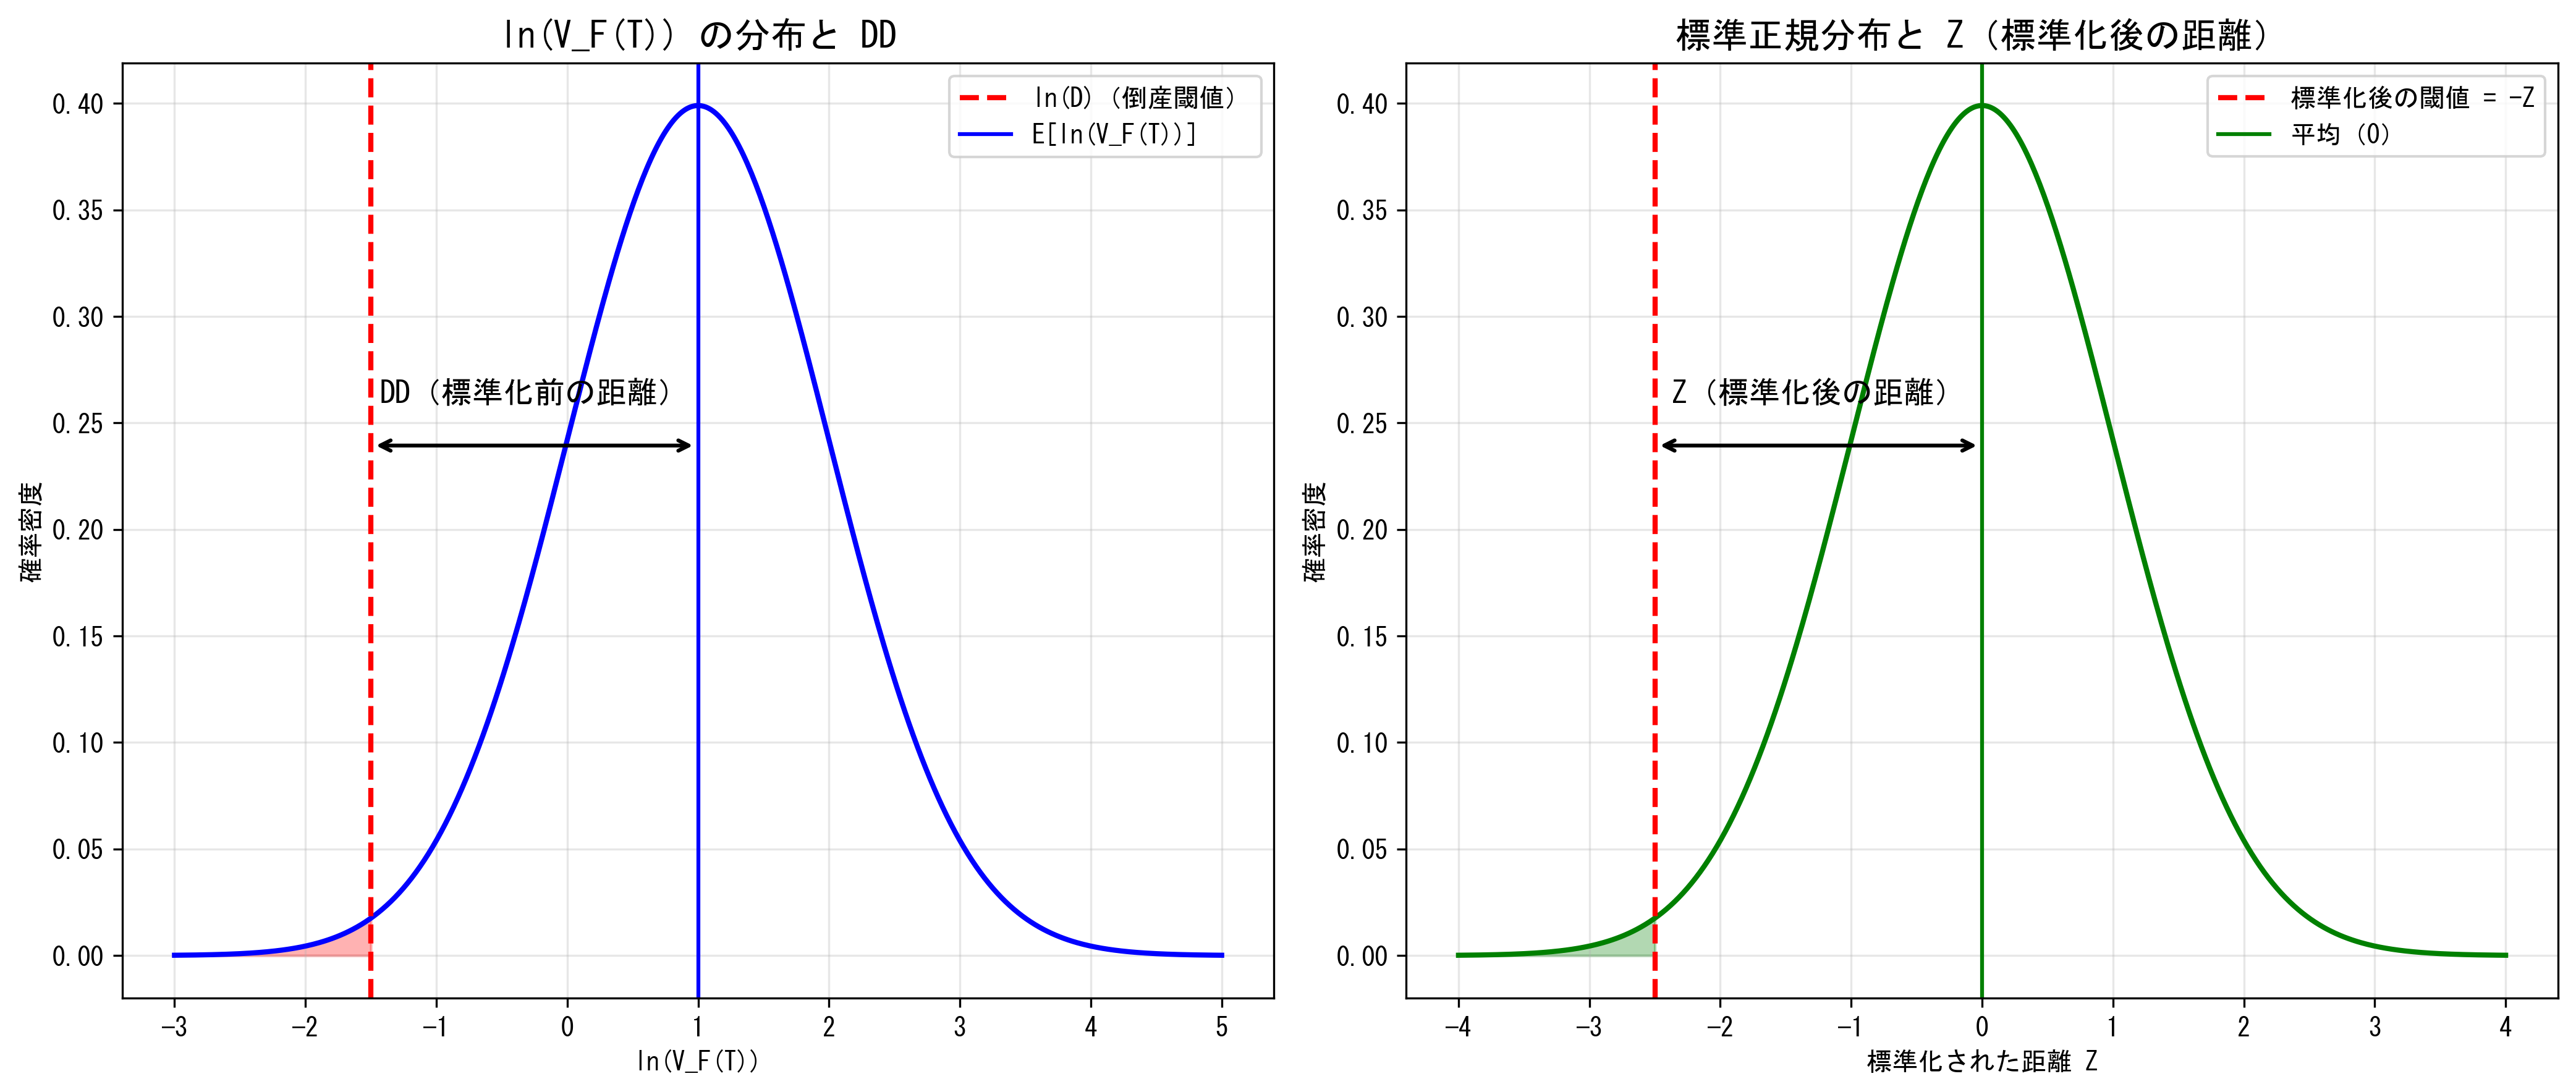
\includegraphics[width=0.85\linewidth]{figures/Bankruptcy_probability_of_Merton_model_with_Z.png}
\caption{
左図は $\ln V_F(T)$ の正規分布における倒産閾値 $\ln D$ と平均 $\mathbb{E}[\ln V_F(T)]$ の距離 DD を示す。
右図は標準正規分布に写像された倒産閾値 $z$ と平均 0 の距離 $z$ を示す。
両図は Merton モデルにおける倒産確率の決定構造（DD → $z$ → $\Phi(-z)$）を視覚的に示している。
}
\end{figure}

\section*{A.2　倒産閾値の標準正規分布への写像}
\addcontentsline{toc}{section}{A.2 倒産閾値の標準正規分布への写像}

Figure 1 の左図では、横軸は $x = \ln V_F(T)$ であり、倒産閾値は



\[
x = \ln D
\]



である。ここで $\ln V_F(T)$ の平均と分散を



\[
\mu_F = \mathbb{E}[\ln V_F(T)], \qquad 
\sigma_F^2 = \mathrm{Var}[\ln V_F(T)]
\]



とおく。

右図は、この分布を標準正規分布へ写像したものであり、横軸は



\[
z = \frac{x - \mu_F}{\sigma_F}
\]



で定義される標準化変数である。したがって倒産閾値 $x = \ln D$ は



\[
z = \frac{\ln D - \mu_F}{\sigma_F}
\]



へと写像される。

一方、倒産距離 DD は



\[
DD = \frac{\mu_F - \ln D}{\sigma_F}
\]



で定義されるため、標準正規分布の座標系では



\[
Z = -DD
\]



と置くことで、倒産方向への距離として解釈できる。

この標準化により、倒産確率は



\[
P(\text{default}) = \Phi(-Z)
\]



として表される。

\section*{A.3　本研究モデルとの対応関係}

本研究では、Merton モデルの構造を財務健全性スコア $F$ と倒産閾値 $\mathrm{Thr}$ に写像することで、
新電力企業の財務データに適用可能な倒産距離モデルを構築する。
このアプローチは Bharath \& Shumway（2008）が示した
「Merton モデルの proxy 化」という考え方を継承している。

\subsection*{（1）財務健全性 $H$ と対数変換 $F$}

本研究では、企業の財務状態を multiplicative に規定する量を「財務健全性」$H$ と定義する。
$H$ は収益性 $\mu$、外部ショック耐性 $\sigma$、支援能力 $S$ など複数の要因が掛け算的に作用する量である。



\[
H = H(\mu, \sigma, S)
\]



multiplicative な構造をもつ $H$ に対して対数変換を施すことで、additive な財務健全性スコア $F$ を得る。



\[
F = \ln H
\]



additive な $F$ は複数要因の和として表現されるため、中心極限定理により正規分布に従うとみなすことができる。

\subsection*{（2）倒産閾値 $\mathrm{Thr}$ の導入}

Merton モデルの倒産閾値 $\ln D$ に対応する量として、財務データに基づき設定される閾値 $\mathrm{Thr}$ を導入する。
財務健全性が閾値を下回る場合に倒産が発生するとみなし、



\[
F \le \mathrm{Thr}
\]



を倒産条件とする。

\subsection*{（3）倒産距離と標準化距離}

倒産距離（Distance to Default, DD）は



\[
DD = F - \mathrm{Thr}
\]



として定義される。さらに、$F$ の標準偏差 $\sigma_F$ で割ることで標準化距離 $Z$ が得られる。



\[
Z = \frac{DD}{\sigma_F}
\]



標準化距離 $Z$ は標準正規分布に従うため、倒産確率は



\[
\pi = \Phi(-Z)
\]



として与えられる。

\begin{figure}[H]
\centering
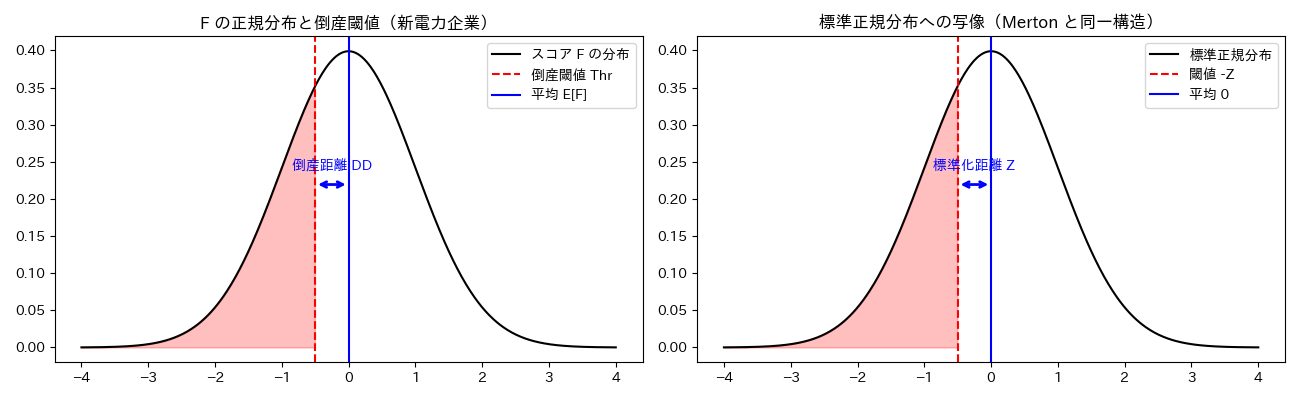
\includegraphics[width=0.95\linewidth]{figures/Bankruptcy_probability_of_New_Power_sec1.png}
\caption{
左図は multiplicative な財務健全性 $H$ を対数変換した財務健全性 $F=\ln H$ の正規分布と倒産閾値 $\mathrm{Thr}$ の関係を示す。
右図は標準正規分布への写像を示し、標準化距離 $Z = DD / \sigma_F$ と倒産確率 $\Phi(-Z)$ の構造が
Merton モデルと同一であることを示している。
}
\end{figure}

\subsection*{（4）対応関係の整理}

\begin{table}[H]
\centering
\begin{tabular}{lll}
\toprule
観点 & Merton モデル & 本研究 \\
\midrule
正規分布に従う変数 & $\ln V_F(T)$ & $F = \ln H$ \\
倒産閾値 & $\ln D$ & $\mathrm{Thr}$ \\
倒産距離（DD） & $E[\ln V_F(T)] - \ln D$ & $F - \mathrm{Thr}$ \\
標準化距離（Z） & $DD / \sigma_{\ln V}$ & $DD / \sigma_F$ \\
倒産確率 & $\Phi(-Z)$ & $\Phi(-Z)$ \\
経済的要因 & $V_F, D, \sigma_V$ & $\mu, \sigma, S$ \\
役割 & 分布を規定 & $H$ の multiplicative 構造を規定 \\
\bottomrule
\end{tabular}
\end{table}

\appendix


% ============================================================
% Appendix B（今回追加する図：ケース別等高線図 & 差分図）
% ============================================================
\chapter*{付録 B：倒産確率の等高線図および差分図}
\addcontentsline{toc}{chapter}{付録 B：倒産確率の等高線図および差分図}

本付録では，第6章で提示した倒産確率サーフェスの補足として，
各ケース（A〜F）の倒産確率 $p$ の等高線図（top view）を示す。
これにより，倒産境界線（$Z_{\text{lin}} = 0$）の形状や，
収益性 $\mu$ と市場ショック $\sigma$ の組み合わせが倒産確率に与える影響を
より直感的に把握できる。
さらに，構造的に意味のある 2 組の比較
（大企業 vs 地方電力，商社系 vs 地域新電力）
について，倒産確率の差分図を示し，
支援能力 $S$ および負債比率 $D$ の影響を定量的に確認する。

% ------------------------------------------------------------
\section*{B.1 ケース別等高線図（A〜F）}
\addcontentsline{toc}{section}{B.1 ケース別等高線図（A〜F）}

以下に，ケースA〜Fの倒産確率 $p$ の等高線図を示す。
いずれも $\mu \in [-0.10, 0.10]$，$\sigma \in [0.05, 0.50]$ の範囲で計算し，
倒産境界線（$Z_{\text{lin}} = 0$）を赤線で強調している。
倒産境界線の位置と形状を比較することで，
負債比率 $D$ と支援能力 $S$ が倒産リスクに与える影響を視覚的に理解できる。

\begin{figure}[H]
    \centering
    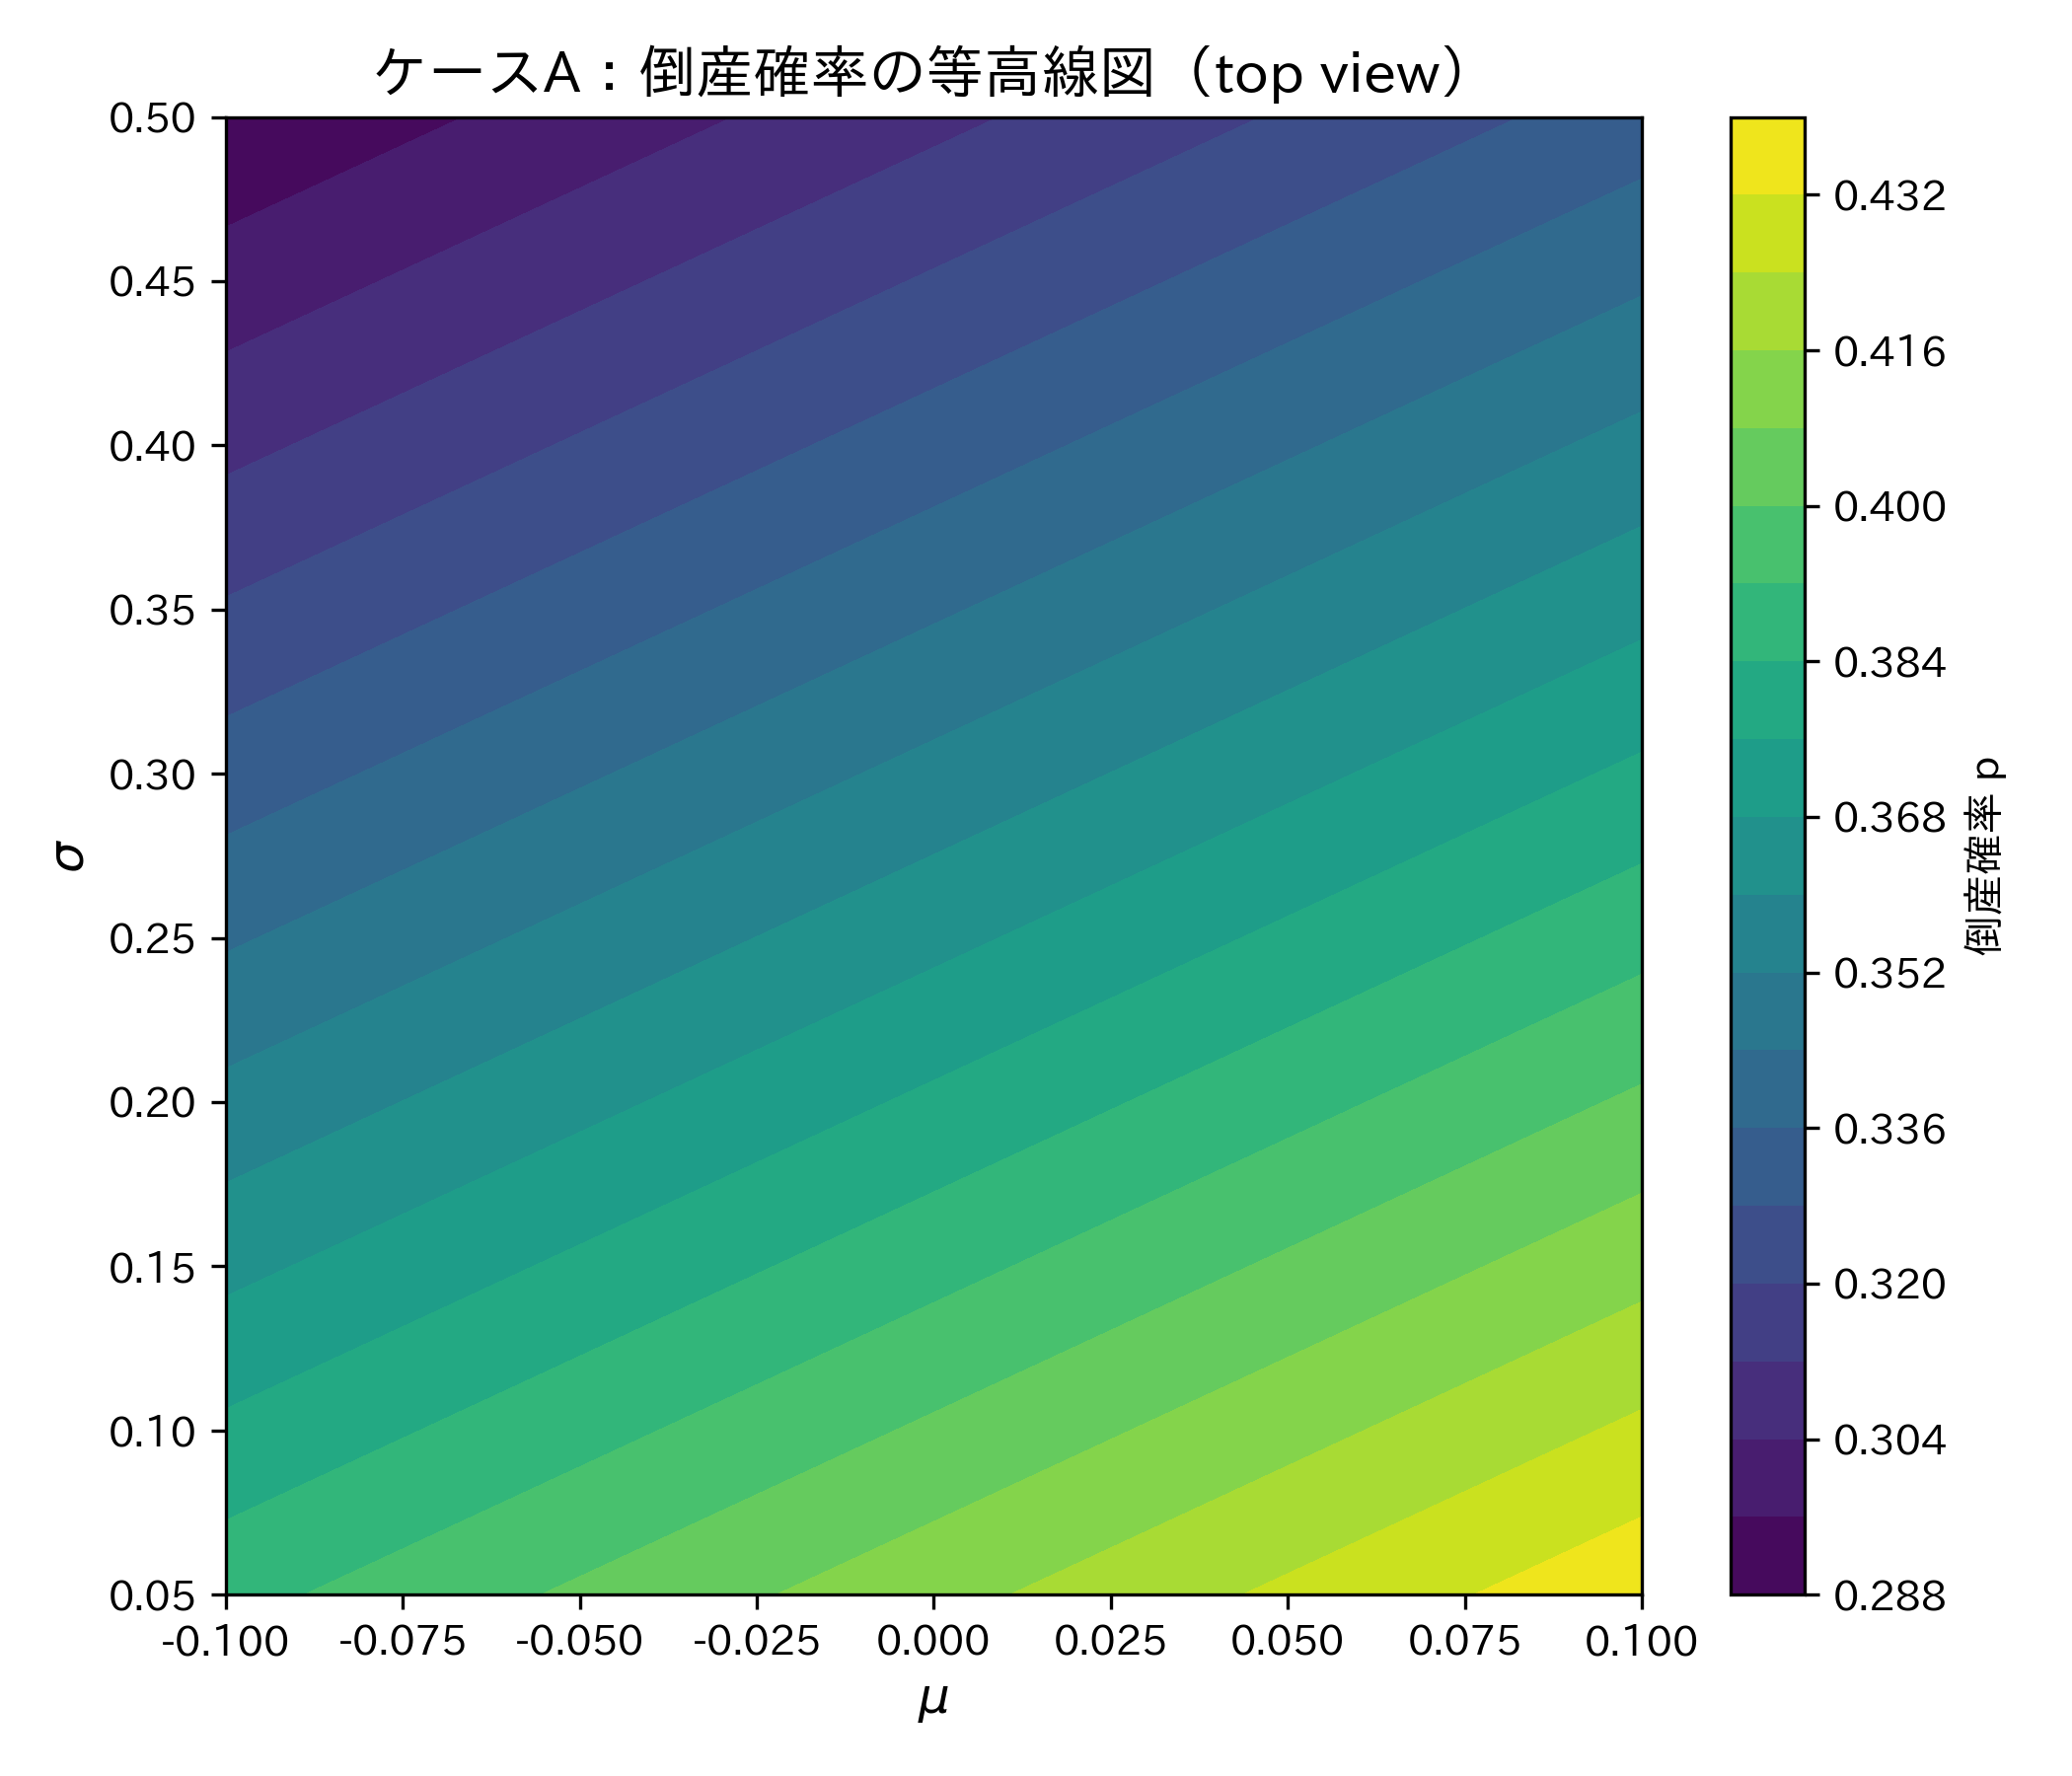
\includegraphics[width=0.75\linewidth]{figures/contour_caseA.png}
    \caption{ケースA（$D=0.3,\ S=0$）：倒産確率の等高線図。
    支援能力がなく，負債比率も低いため，境界線は中間的な位置にある。}
\end{figure}

\begin{figure}[H]
    \centering
    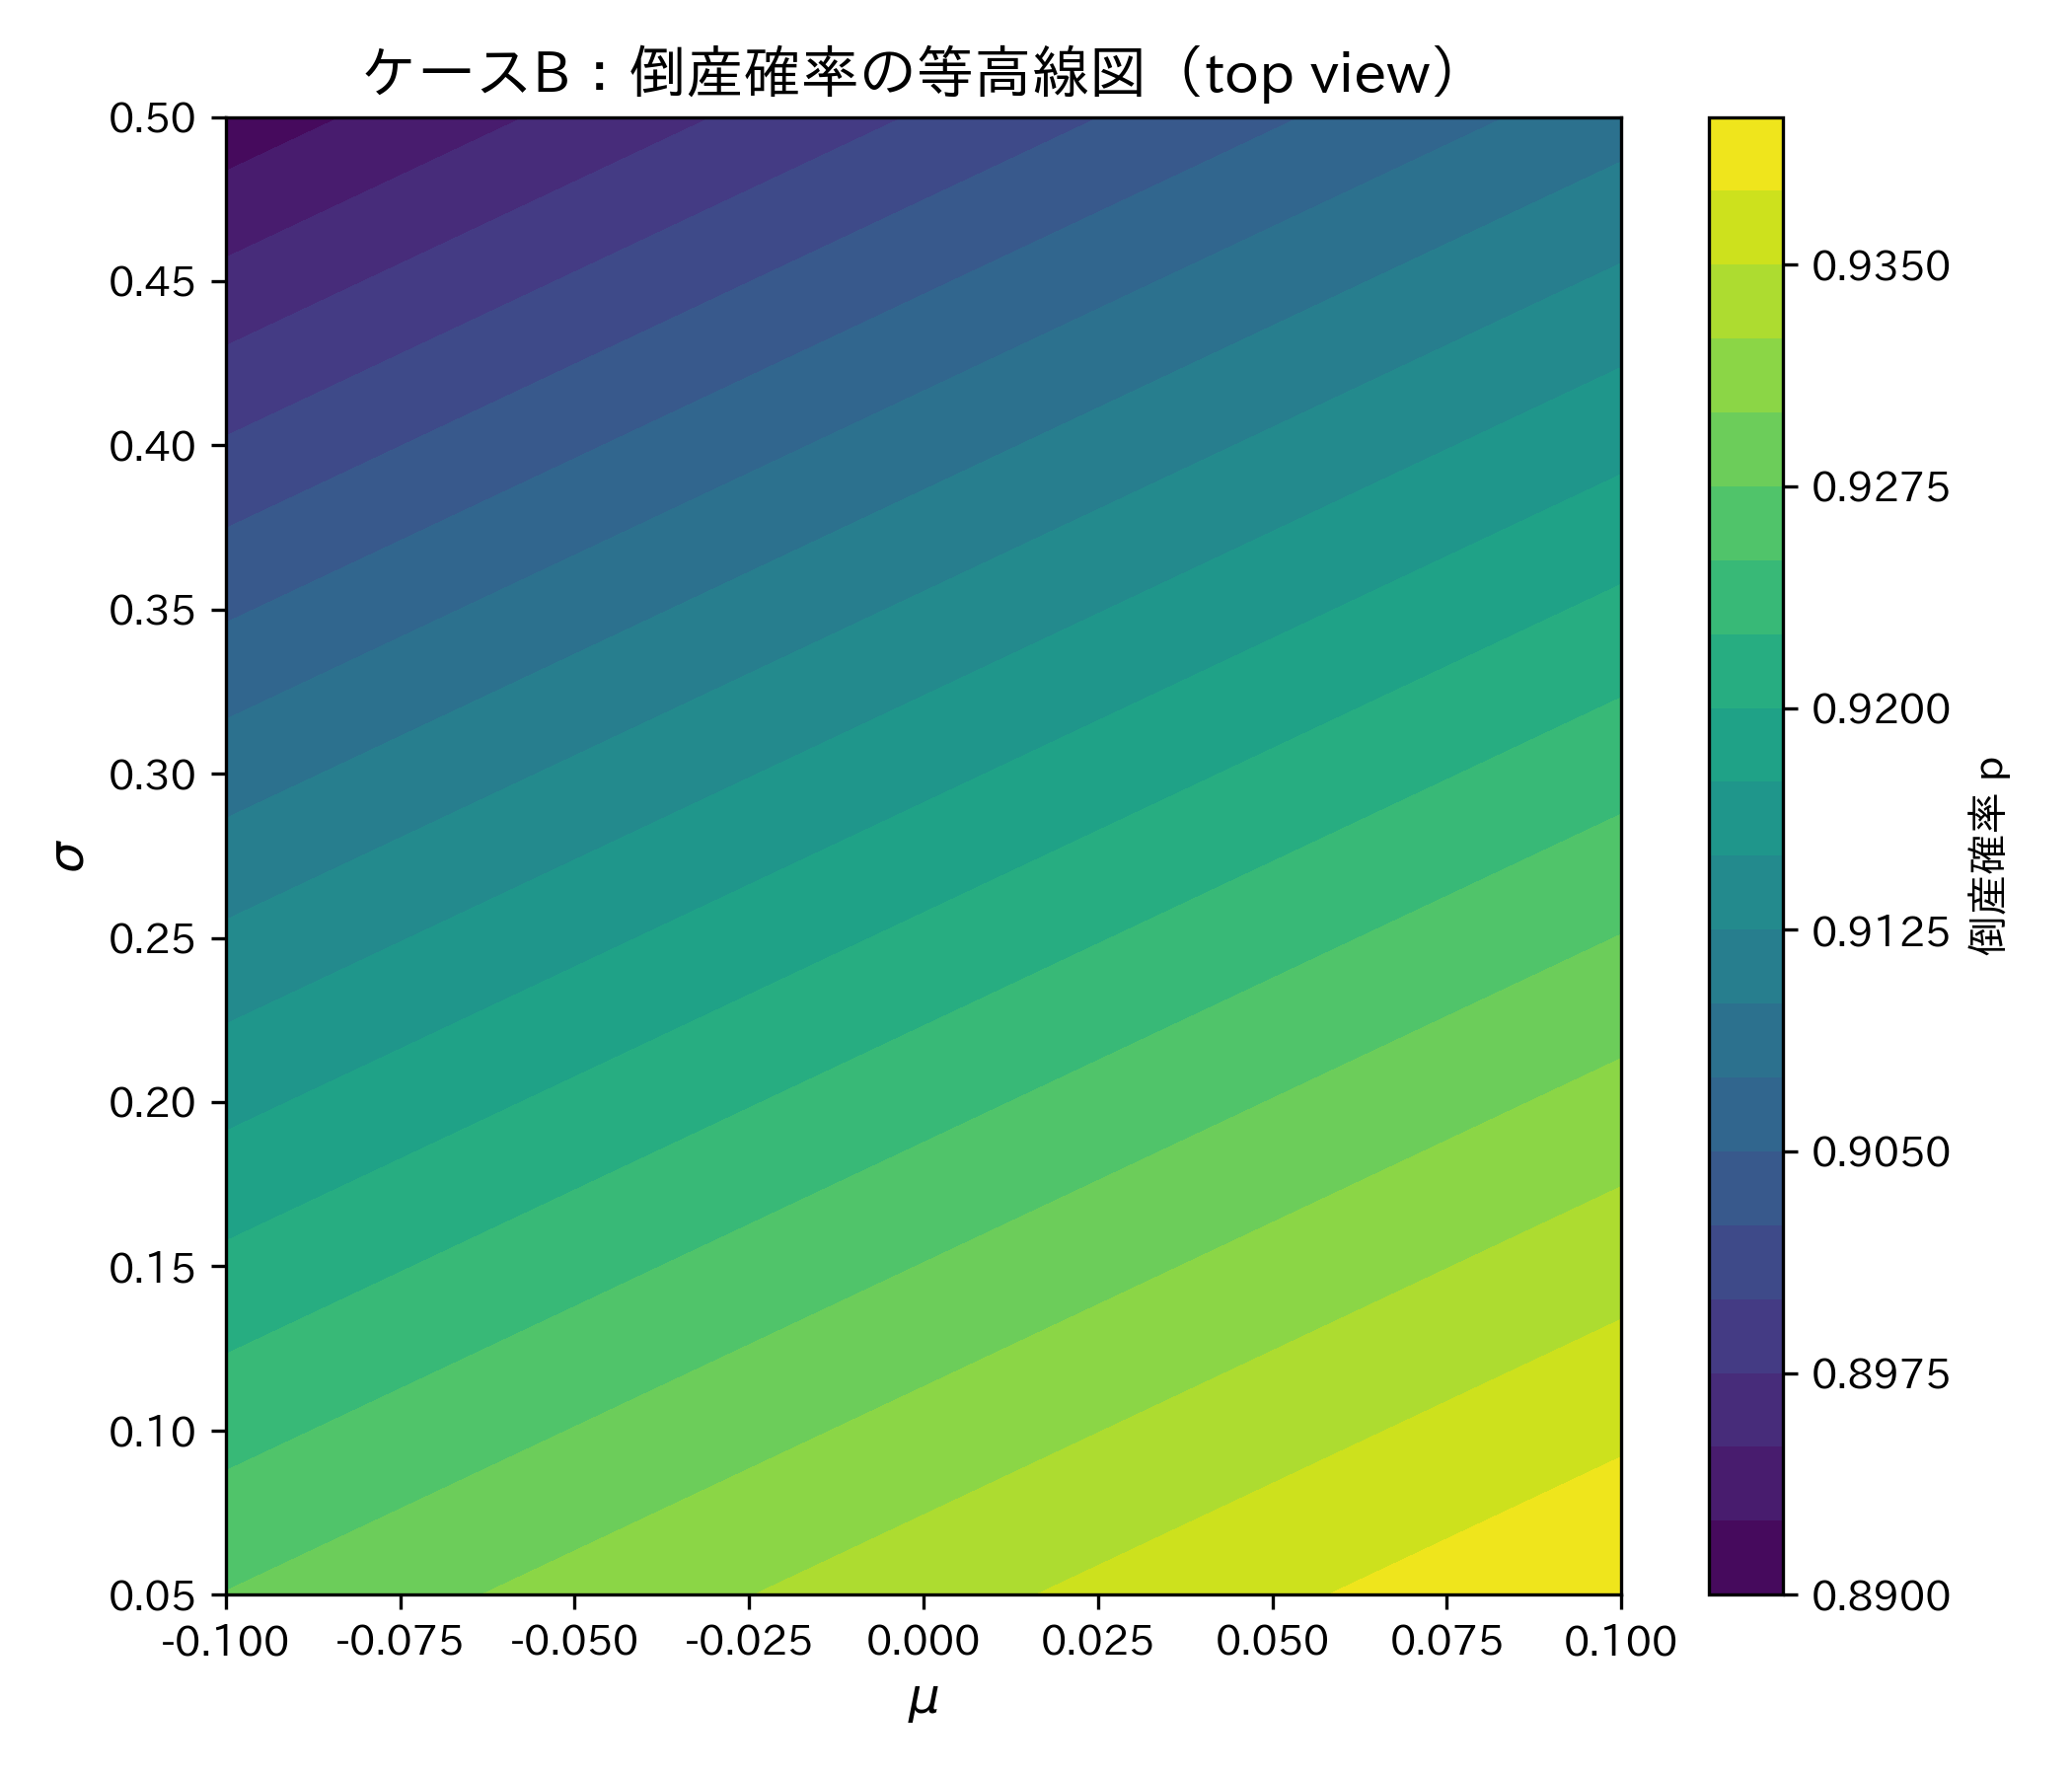
\includegraphics[width=0.75\linewidth]{figures/contour_caseB.png}
    \caption{ケースB（$D=0.3,\ S=3$）：倒産確率の等高線図。
    強い支援能力により倒産境界線が大きく右へ移動し，
    市場ショックに対する耐性が高いことがわかる。}
\end{figure}

\begin{figure}[H]
    \centering
    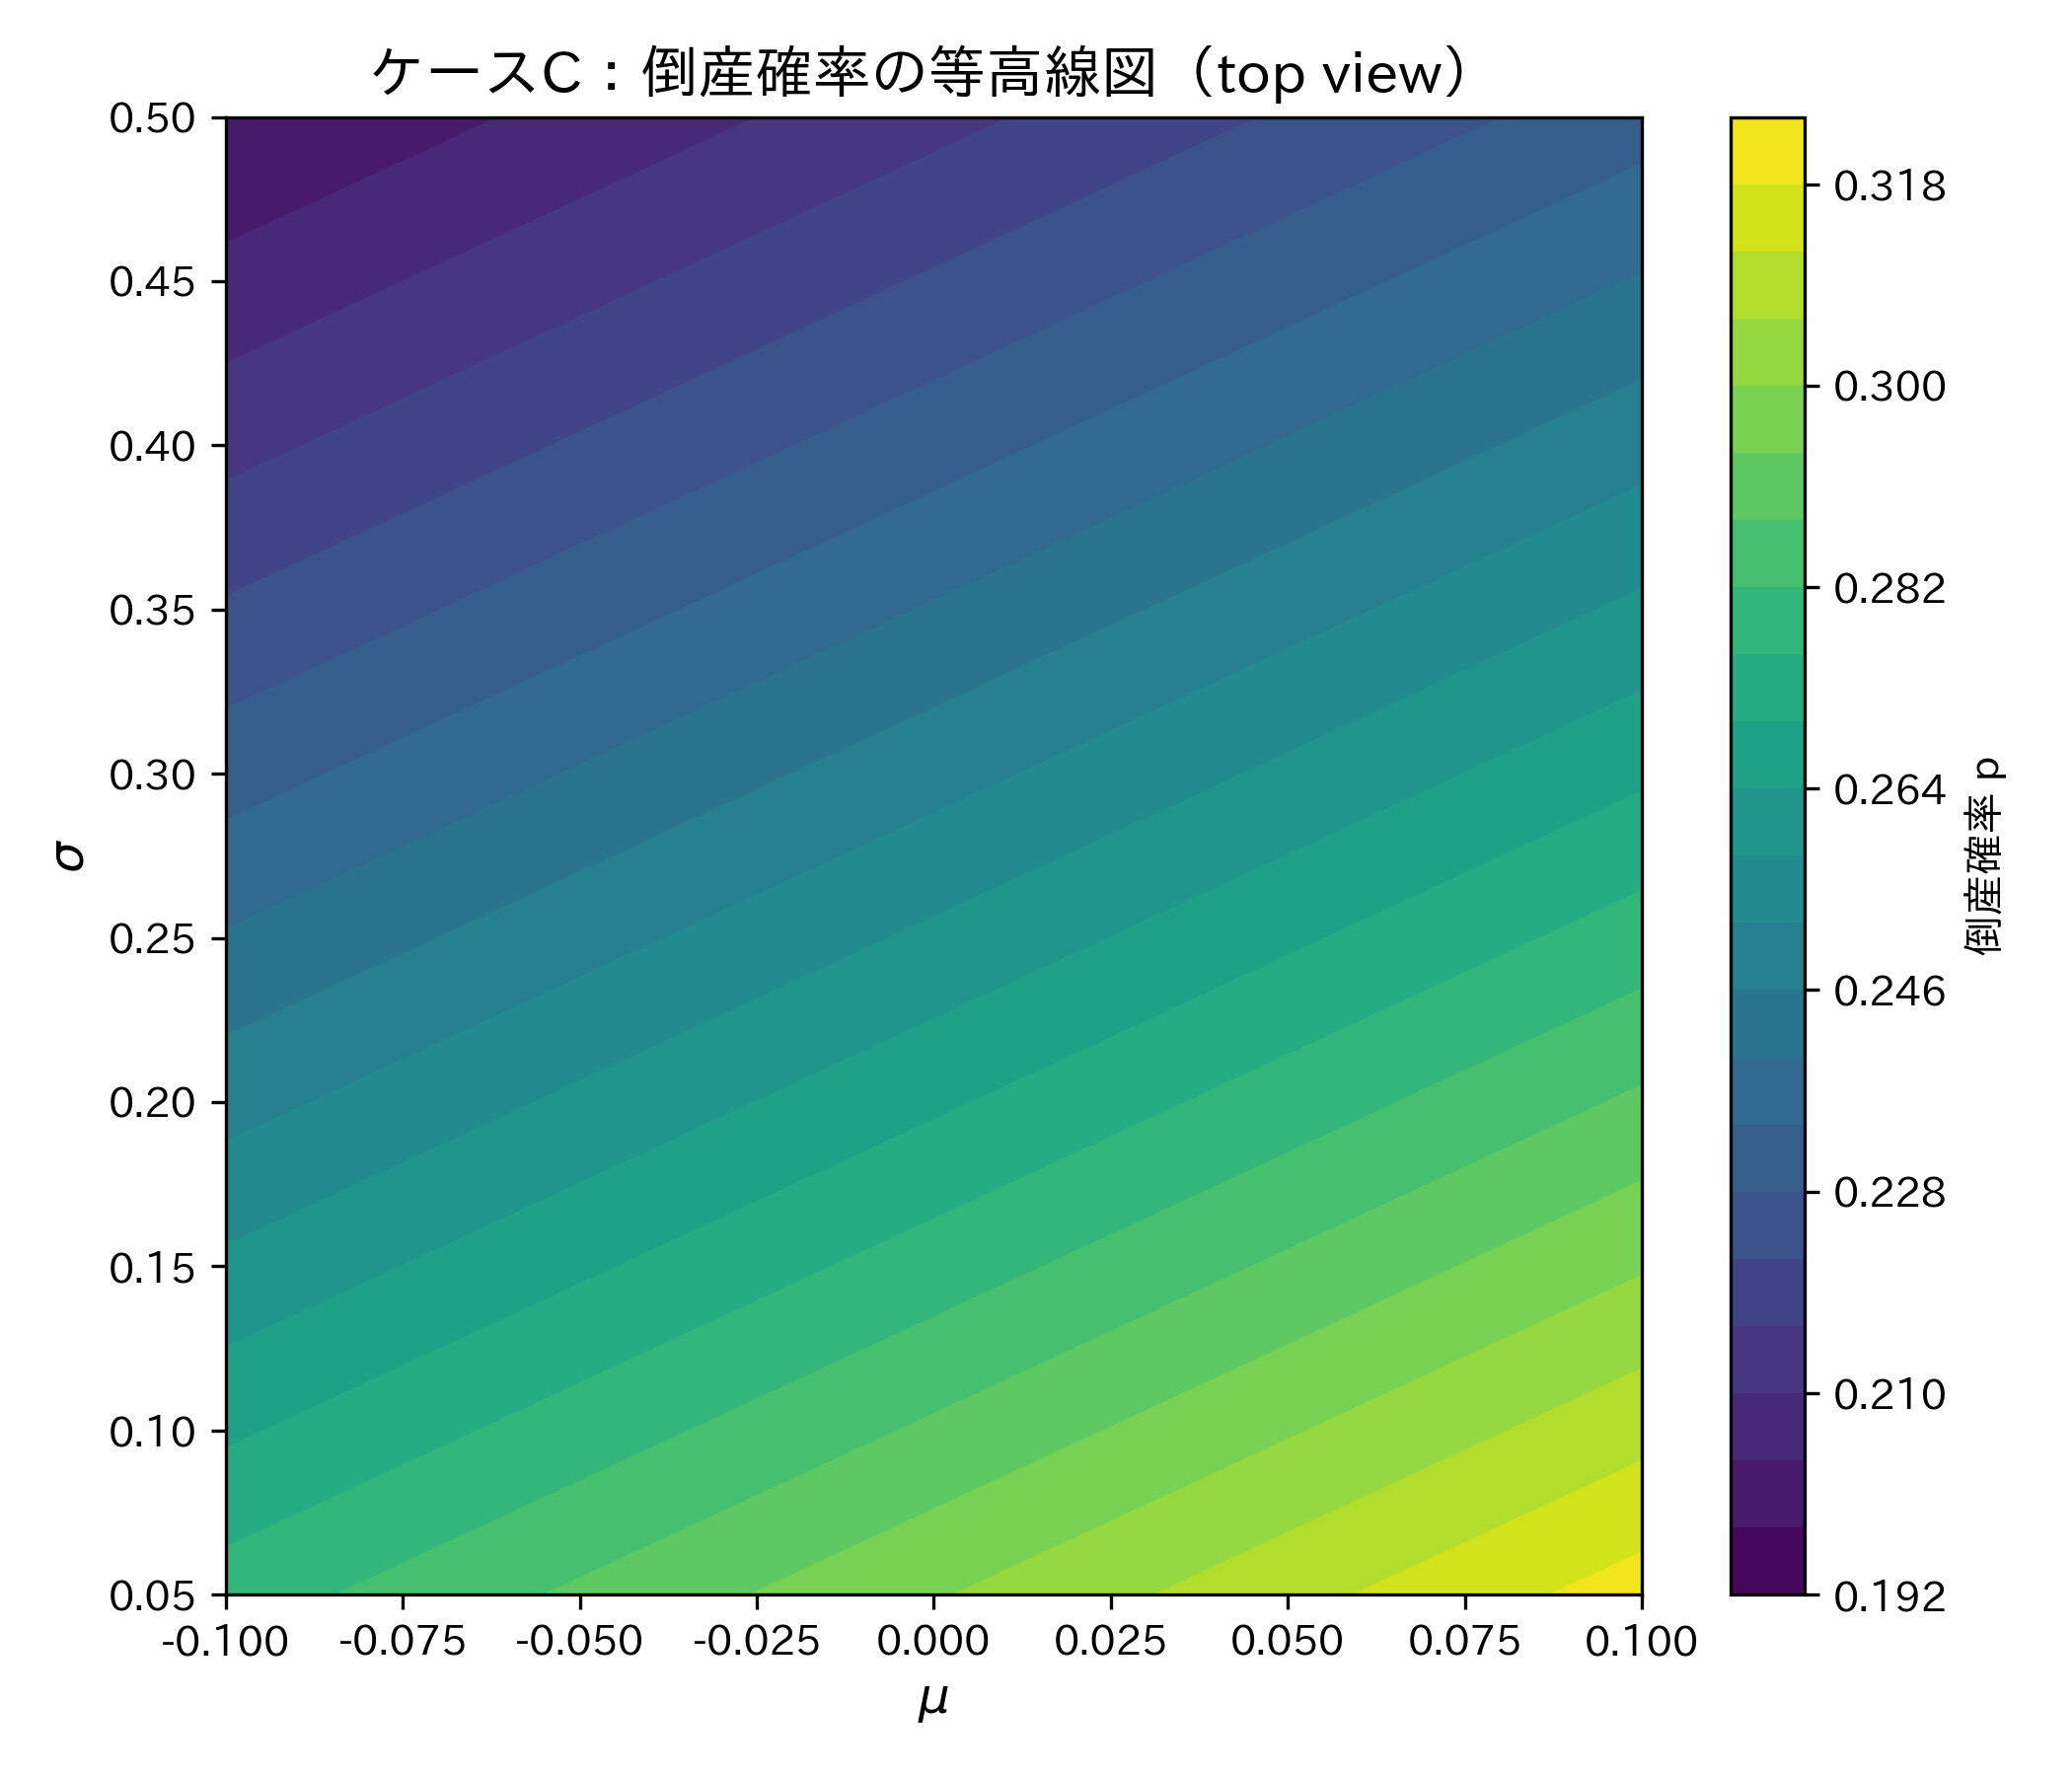
\includegraphics[width=0.75\linewidth]{figures/contour_caseC.png}
    \caption{ケースC（$D=0.8,\ S=0$）：倒産確率の等高線図。
    負債過多により境界線が大きく左へ寄り，
    高ボラティリティ環境で極めて脆弱であることが示される。}
\end{figure}

\begin{figure}[H]
    \centering
    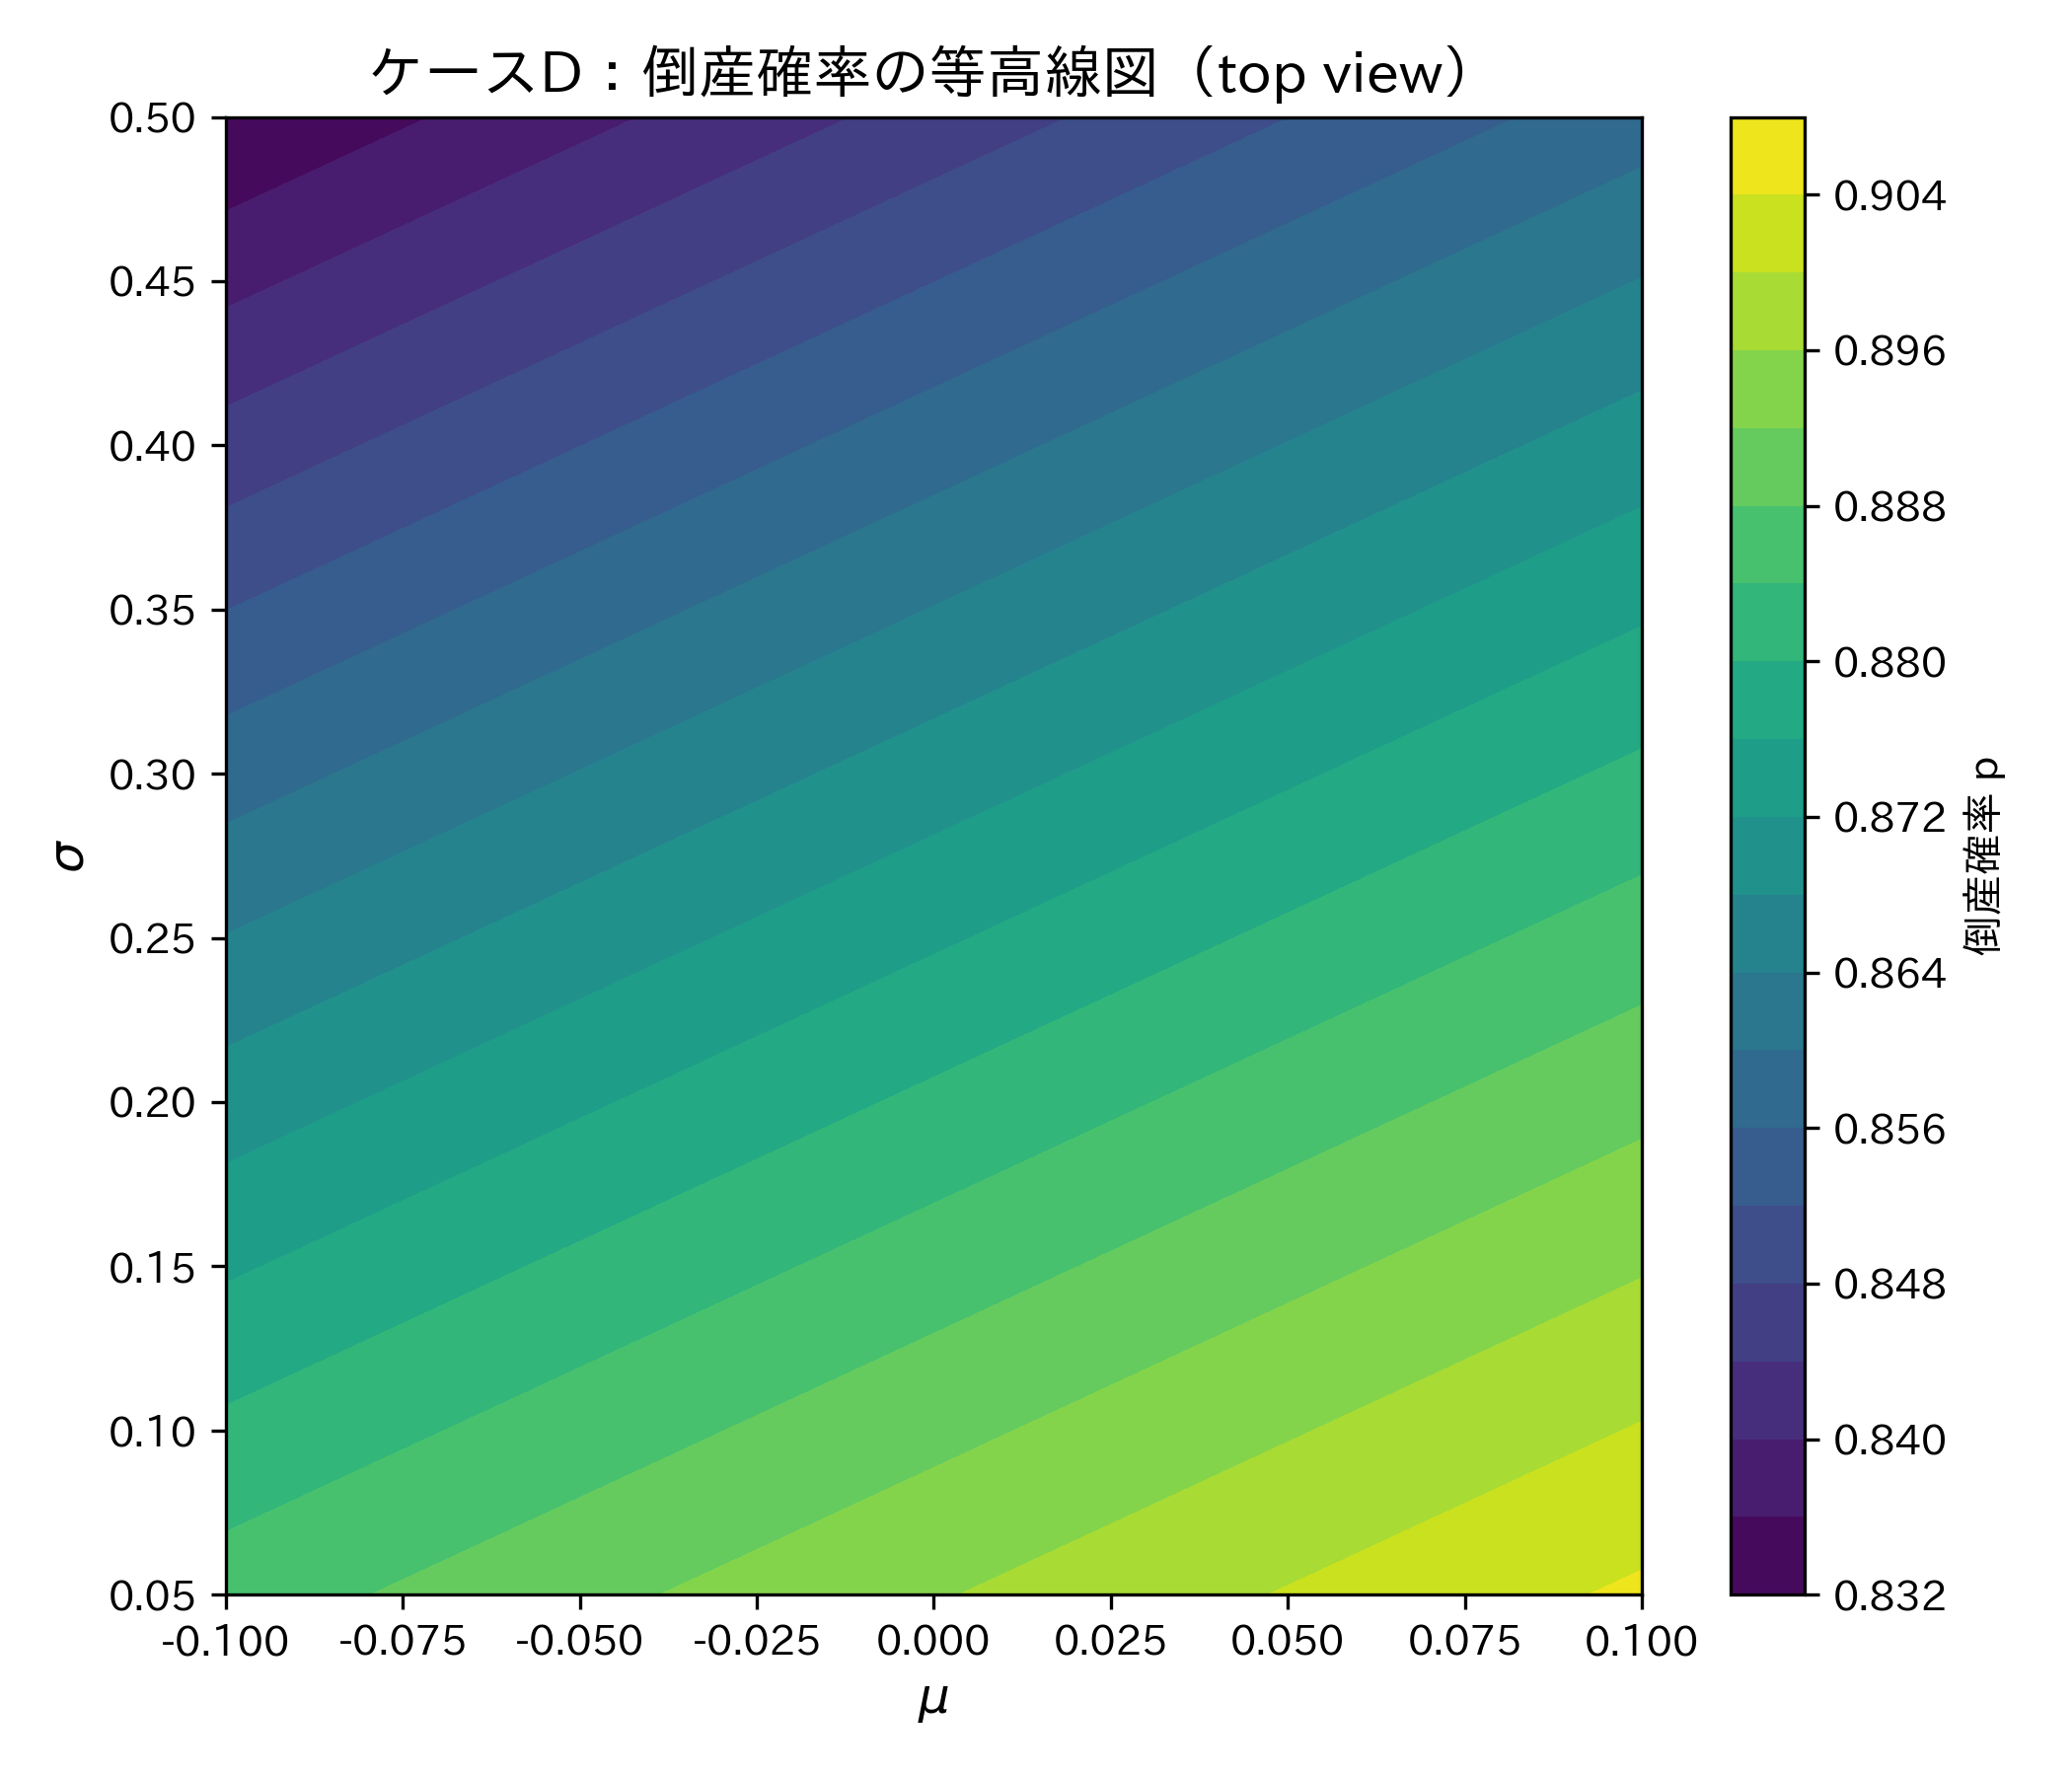
\includegraphics[width=0.75\linewidth]{figures/contour_caseD.png}
    \caption{ケースD（$D=0.8,\ S=3$）：倒産確率の等高線図。
    負債比率は高いが支援能力が強いため，
    ケースCと比べて境界線が右へ戻り，倒産リスクが大幅に緩和されている。}
\end{figure}

\begin{figure}[H]
    \centering
    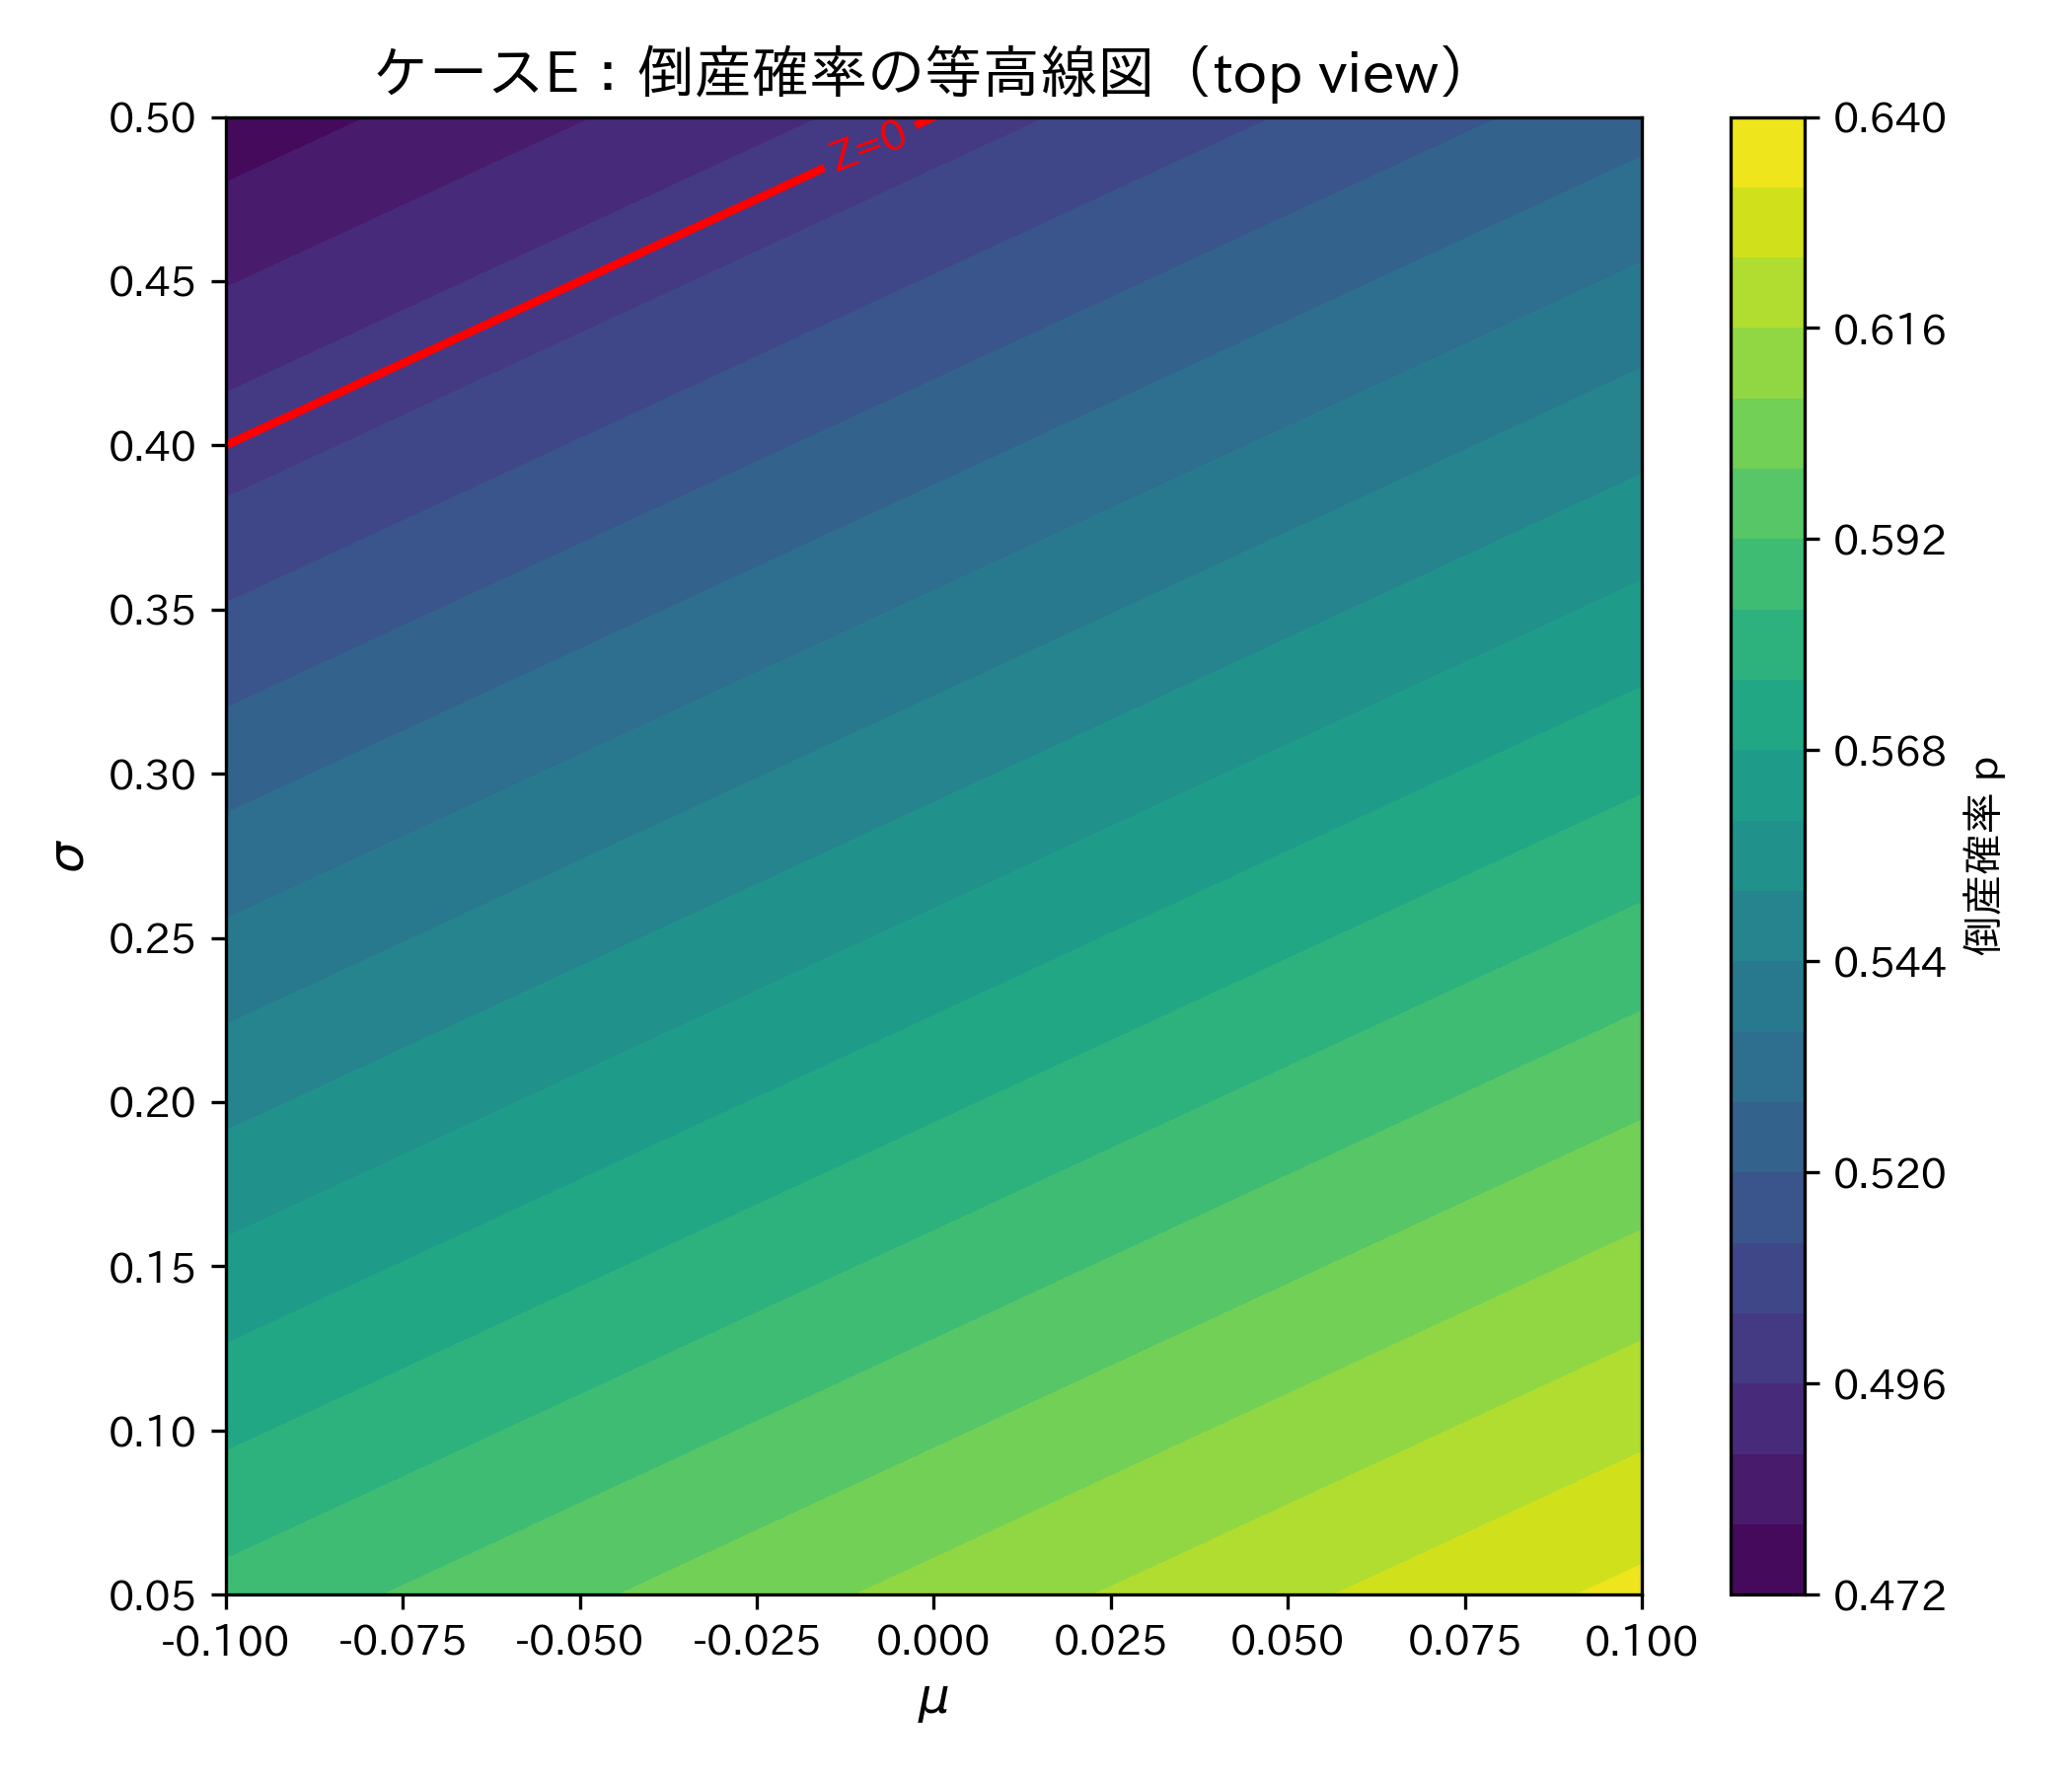
\includegraphics[width=0.75\linewidth]{figures/contour_caseE.png}
    \caption{ケースE（$D=0.5,\ S=1$）：倒産確率の等高線図。
    地域新電力の典型であり，収益性と市場ショックに敏感な構造が確認できる。}
\end{figure}

\begin{figure}[H]
    \centering
    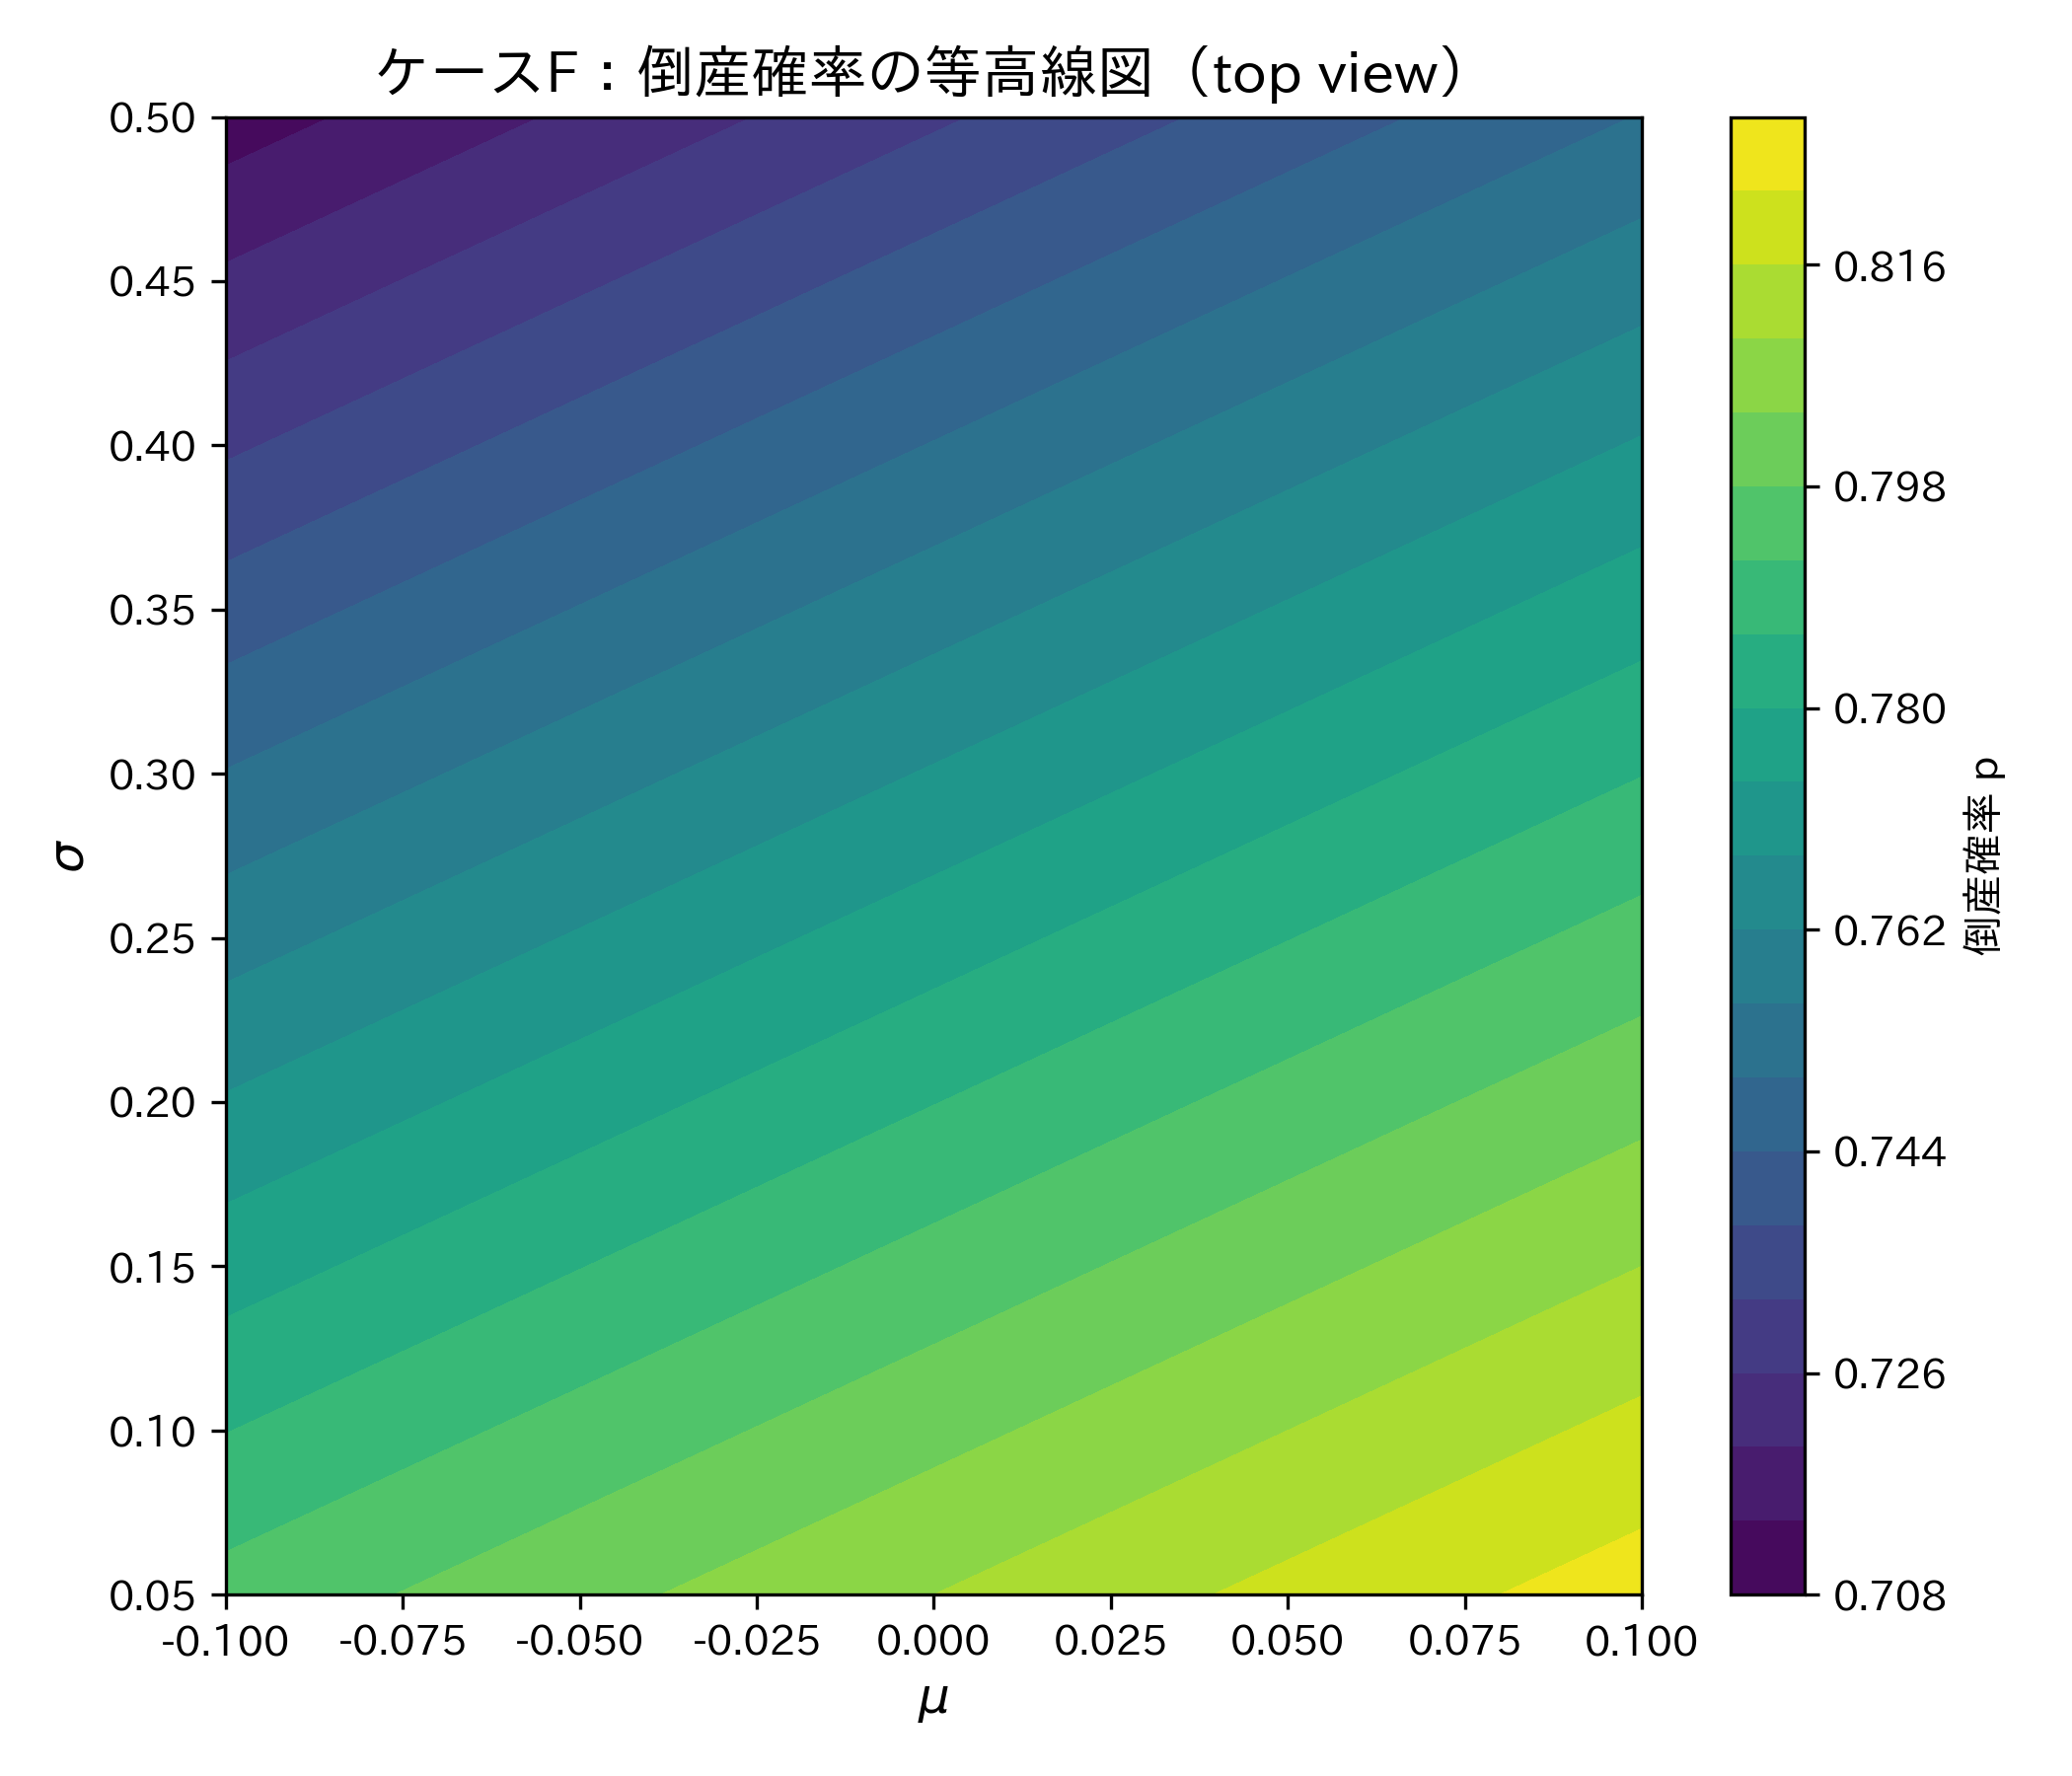
\includegraphics[width=0.75\linewidth]{figures/contour_caseF.png}
    \caption{ケースF（$D=0.5,\ S=2$）：倒産確率の等高線図。
    ケースEと比べて境界線が右へ移動し，
    支援能力の差が倒産リスクを大きく左右することが視覚的に示される。}
\end{figure}

% ------------------------------------------------------------
\section*{B.2 差分図（B−C および F−E）}
\addcontentsline{toc}{section}{B.2 差分図（B−C および F−E）}

本節では，構造的に意味のある 2 組の比較について，
倒産確率の差分 $\Delta p$ を可視化する。
差分図は，支援能力 $S$ と負債比率 $D$ の違いが
倒産確率にどの程度の差を生むかを定量的に示すものである。

\subsection*{B.2.1 大企業 vs 地方電力（ケースB − ケースC）}


\[
\Delta p = p_{\mathrm{B}} - p_{\mathrm{C}}
\]



\begin{figure}[H]
    \centering
    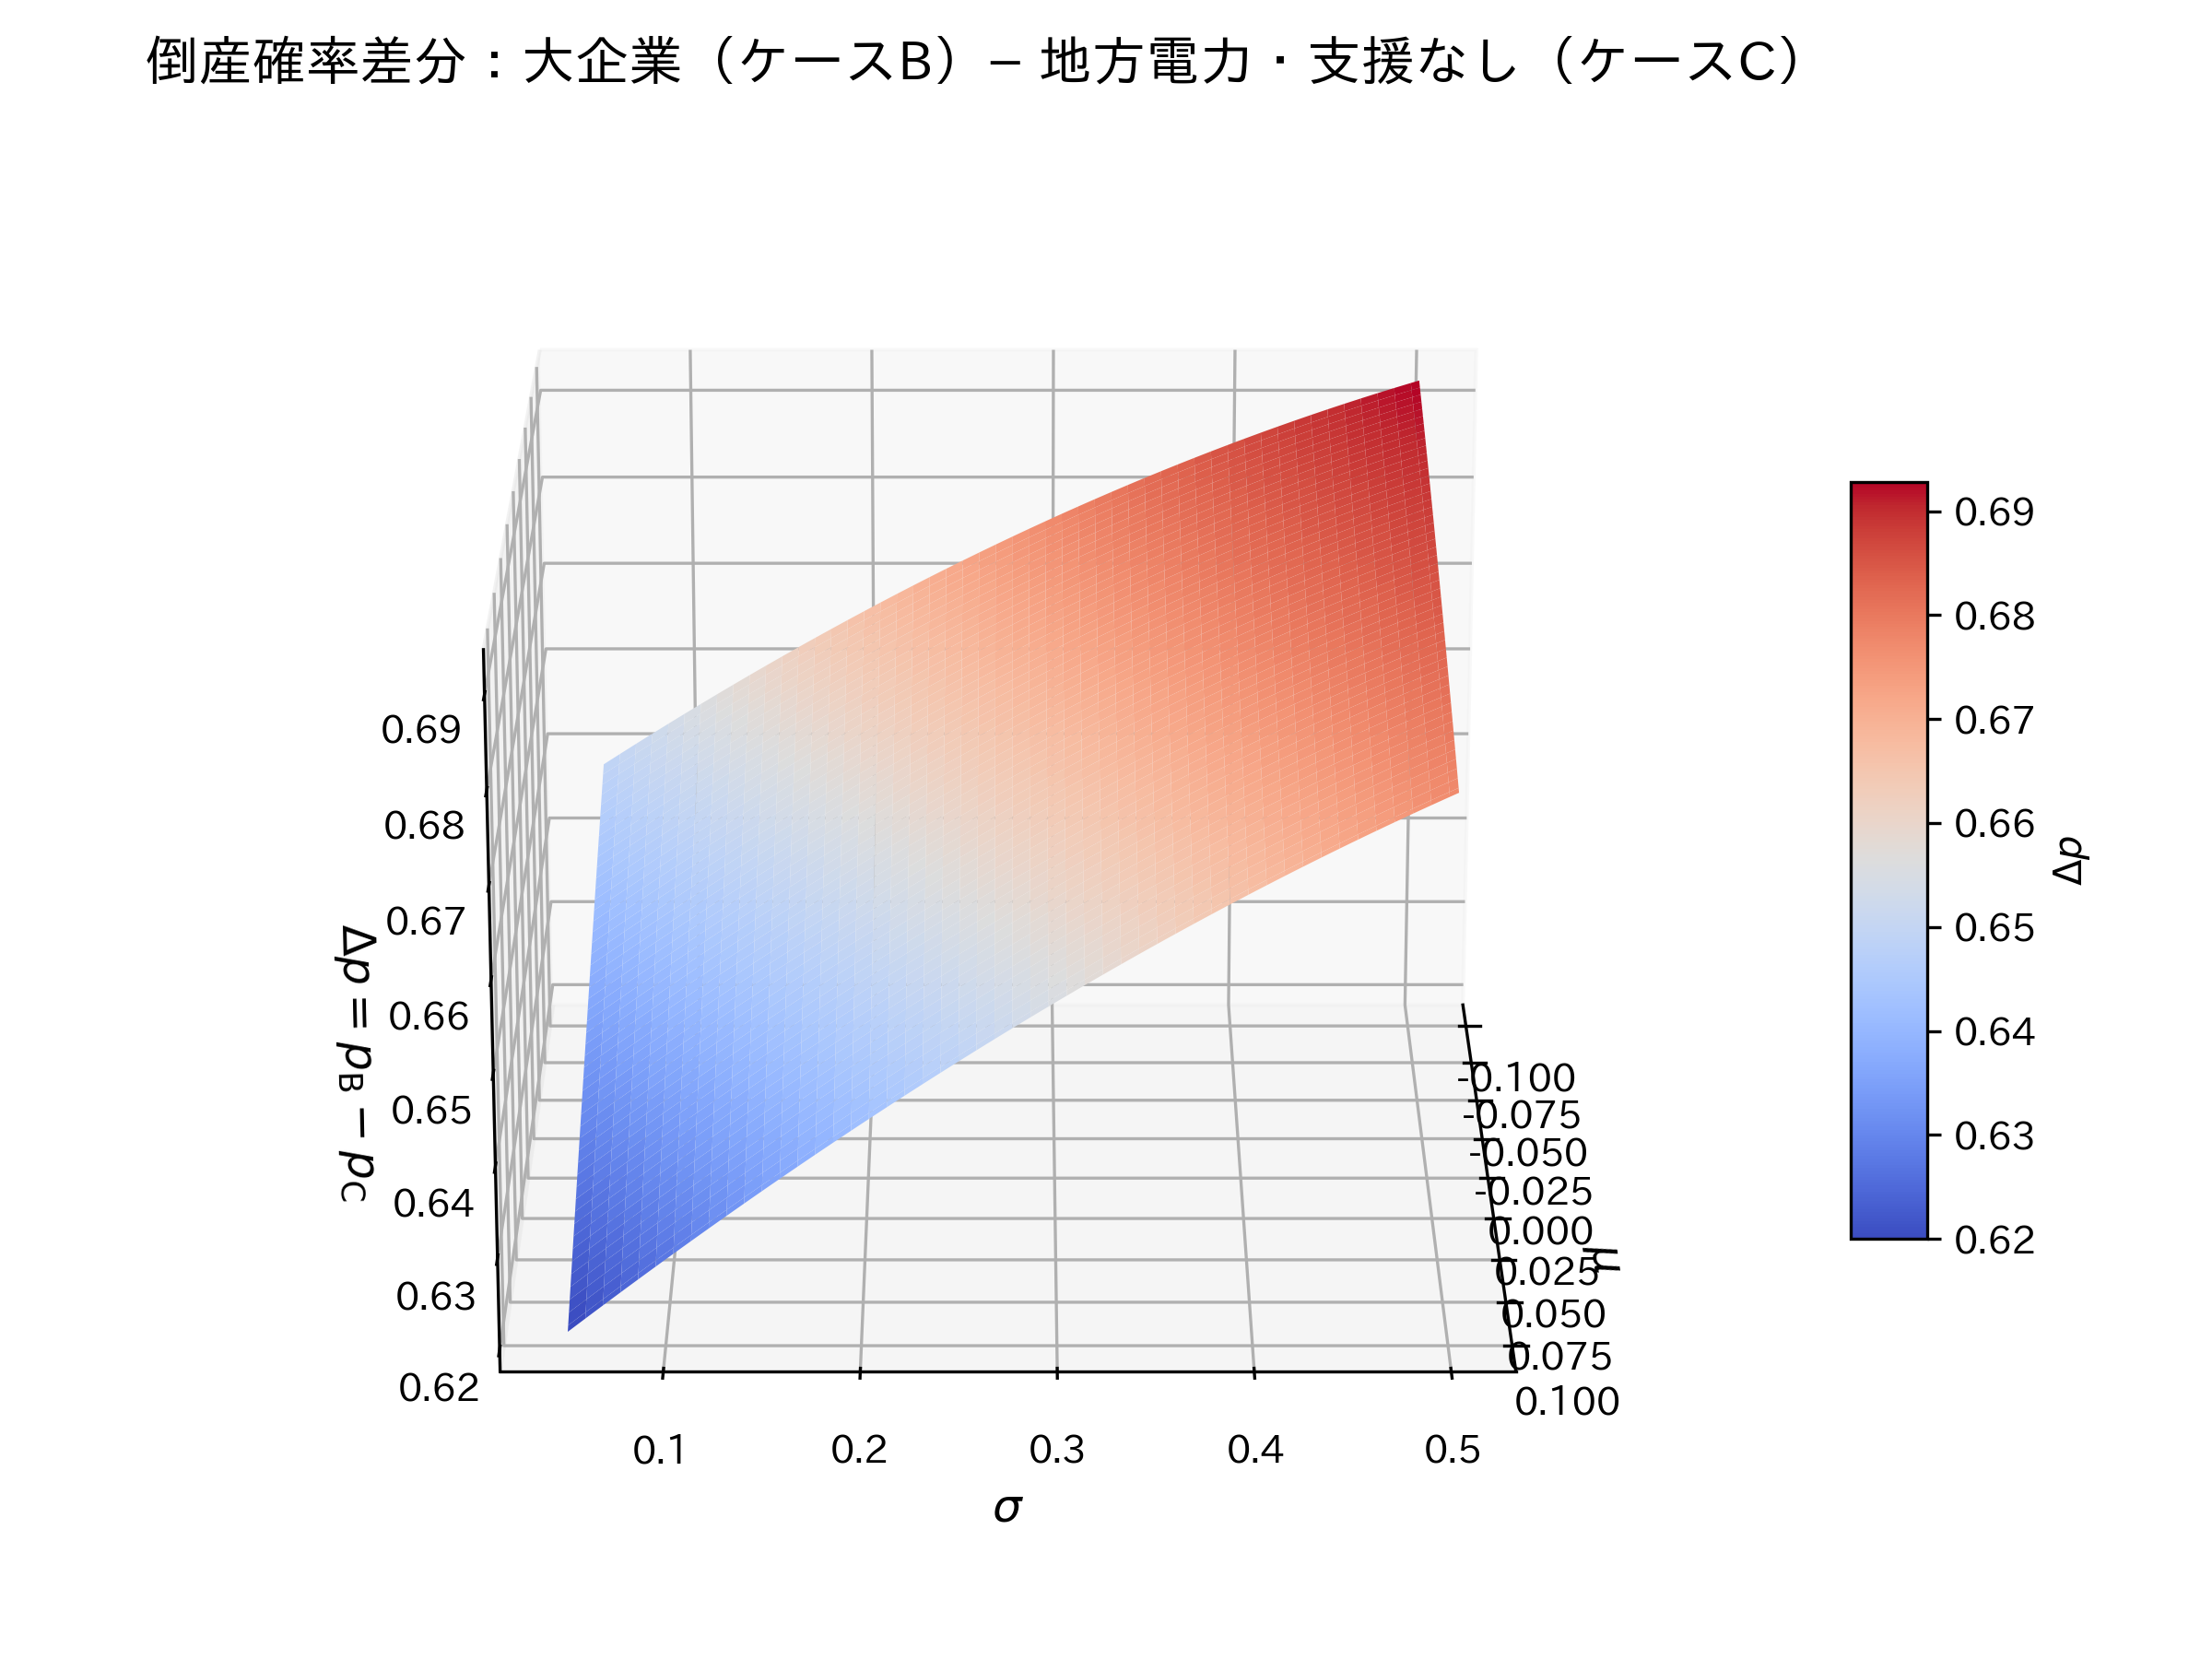
\includegraphics[width=0.75\linewidth]{figures/surface_diff_B_minus_C.png}
    \caption{倒産確率差分：大企業（ケースB）$-$ 地方電力（ケースC）。
    全域で $\Delta p > 0$ となり，支援能力の有無が倒産確率に
    決定的な差を生むことが確認できる。}
\end{figure}

\subsection*{B.2.2 商社系 vs 地域新電力（ケースF − ケースE）}


\[
\Delta p = p_{\mathrm{F}} - p_{\mathrm{E}}
\]



\begin{figure}[H]
    \centering
    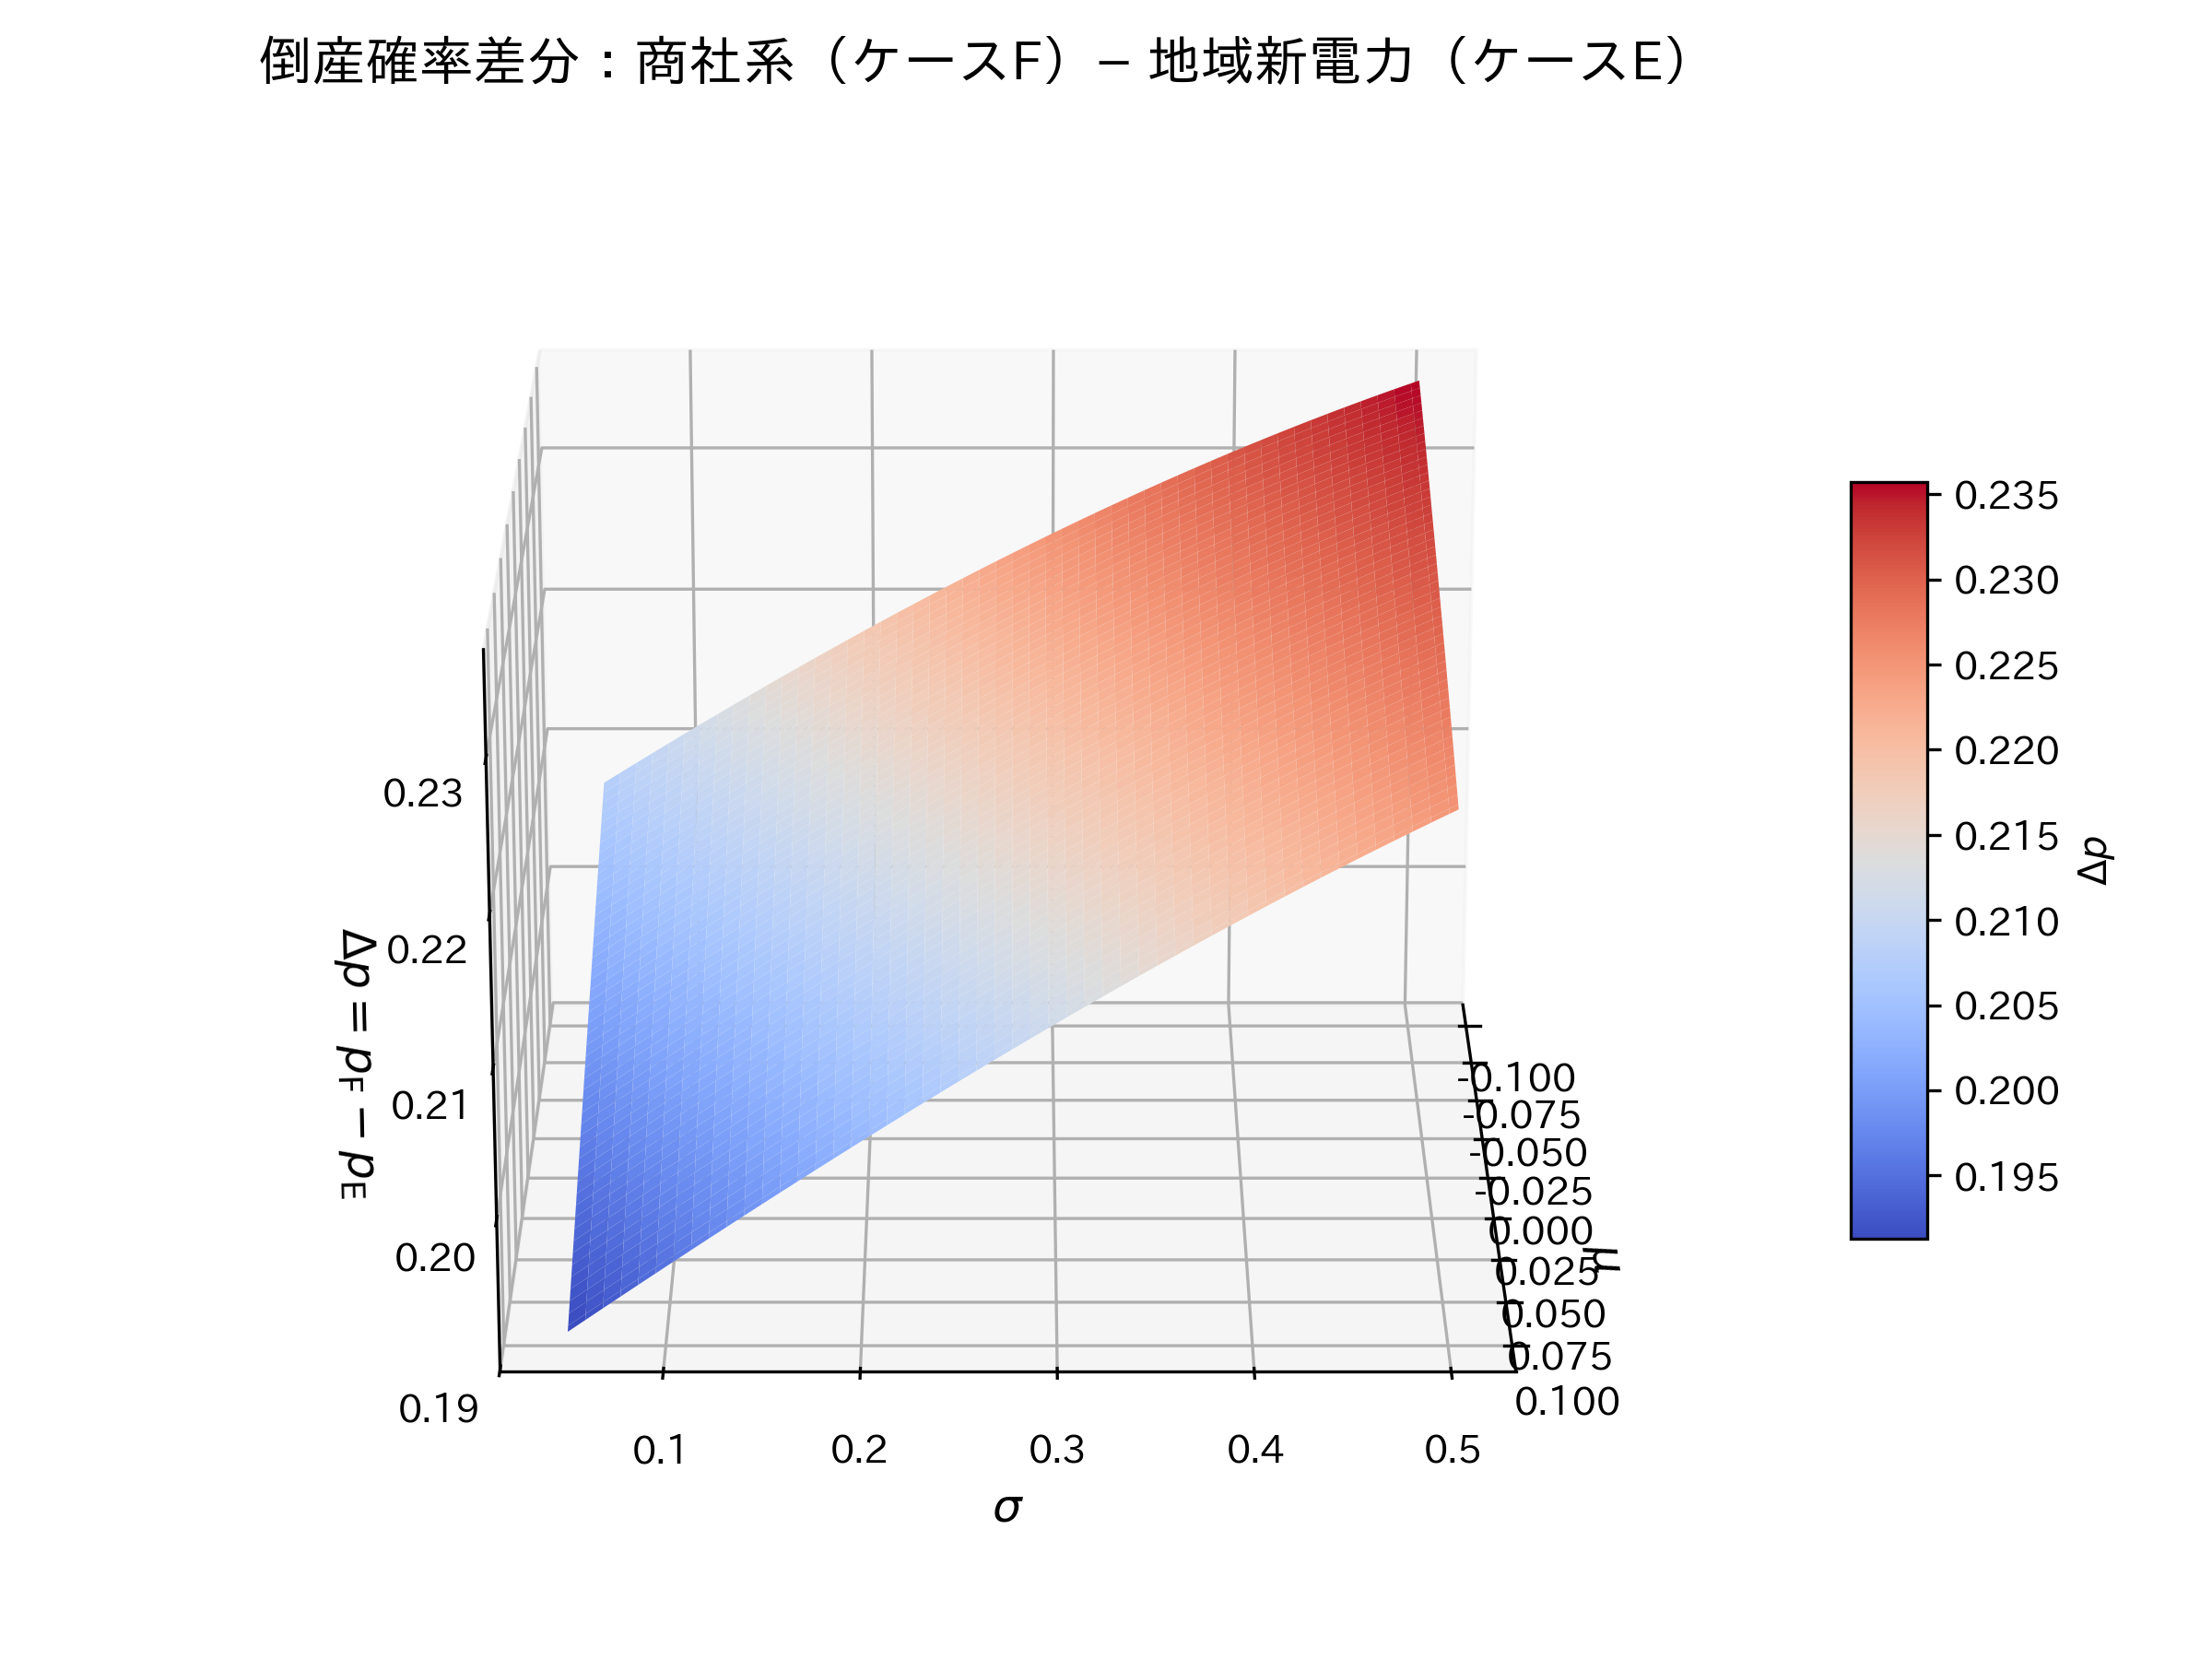
\includegraphics[width=0.75\linewidth]{figures/surface_diff_F_minus_E.png}
    \caption{倒産確率差分：商社系（ケースF）$-$ 地域新電力（ケースE）。
    支援能力 $S$ の差が倒産確率に 0.2〜0.3 程度の差を生み，
    特に $\sigma$ が大きい領域でその効果が最大化する。}
\end{figure}

以上の差分図は，第6章で議論したとおり，
支援能力 $S$ および負債比率 $D$ が倒産確率に与える影響を
視覚的かつ定量的に示すものである。
特に，ケースF−E の比較は，
中規模企業における支援能力の重要性を明確に示している。

% ============================================================
% 付録C B&S 推定式に基づく proxy 妥当性シミュレーション
% ------------------------------------------------------------
% ・第5章で定義した proxy（μ, σ, S, D）がどの程度「真の構造」を回収できるかを検証
% ・理論モデル（真の世界）→ proxy（観測世界）→ B&S 型ロジット推定 の流れを再現
% ・第7章の実証分析に向けた proxy 妥当性の理論的裏付けを与える
% ============================================================

\chapter*{付録 C：B\&S 推定式に基づく proxy 妥当性シミュレーション}
\label{app:bs_simulation}

\section*{C.1　B\&S 推定式に基づく proxy 妥当性シミュレーション}

本節では，第5章で定義した収益性 $\mu$，市場ショック $\sigma$，
支援能力 $S$，倒産閾値 $D$ の各 proxy が，
理論モデルの「真の構造」をどの程度回収できるかを検証するため，
Bharath and Shumway（2008）（以下 B\&S）の推定式に基づく
シミュレーション分析を行う。

本分析の目的は，実証データが限定的な新電力企業において，
proxy 変数を用いたロジット推定がどの程度信頼できるかを
理論的に裏付けることである。

% ------------------------------------------------------------
\subsection*{C.1.1　分析の基本構造：真の世界と観測世界}

本シミュレーションは，以下の 3 段階で構成される。

\begin{enumerate}
    \item \textbf{真の世界（理論モデル）}  
    第4章で導出した潜在倒産距離
    


\[
        Z^{\ast}_i = a \mu^{\ast}_i - b \sigma^{\ast}_i + c S^{\ast}_i - d D^{\ast}_i
    \]



    を用いて，真の倒産確率
    


\[
        p_i = \frac{1}{1 + \exp(-Z^{\ast}_i)}
    \]



    を生成し，倒産ダミー $\text{Default}_i$ を発生させる。

    \item \textbf{観測世界（proxy の生成）}  
    真のパラメータ $\mu^{\ast}, \sigma^{\ast}, S^{\ast}, D^{\ast}$ から，
    第5章で定義した観測可能な proxy を生成する。

    \item \textbf{B\&S 型ロジット推定}  
    観測 proxy を説明変数としてロジット推定を行い，
    真の係数 $(a,b,c,d)$ をどの程度回収できるかを比較する。
\end{enumerate}

% ------------------------------------------------------------
\subsection*{C.1.2　真のパラメータの設定}

真のパラメータは以下のように設定する。



\[
\mu^{\ast}_i \sim N(0.02, 0.03^2), \qquad
\sigma^{\ast}_i \sim N(0.20, 0.05^2)
\]





\[
S^{\ast}_i \in \{0,1,2,3\}, \qquad
D^{\ast}_i \sim \mathrm{Lognormal}(-1.0, 0.4^2)
\]



係数は理論モデルの符号条件に基づき，



\[
a = 1.0,\quad b = 1.0,\quad c = 0.8,\quad d = 1.2
\]



とする。

% ------------------------------------------------------------
\subsection*{C.1.3　proxy の生成：観測誤差の導入}

\noindent\textbf{（1）収益性の proxy}



\[
\tilde{\mu}^{(1)}_i = \mu^{\ast}_i + \varepsilon^{(1)}_i
\qquad
\tilde{\mu}^{(2)}_i = 0.8 \mu^{\ast}_i + \varepsilon^{(2)}_i
\]



\noindent\textbf{（2）市場ショックの proxy}



\[
\tilde{\sigma}_i = 0.7 \sigma^{\ast}_i + \eta_i
\]



\noindent\textbf{（3）支援能力の proxy}



\[
\tilde{S}_i =
\begin{cases}
S^{\ast}_i & \text{確率 } 0.9 \\
S^{\ast}_i - 1 & \text{確率 } 0.1
\end{cases}
\]



\noindent\textbf{（4）倒産閾値の proxy}



\[
\tilde{D}_i = D^{\ast}_i + \xi_i
\]



% ------------------------------------------------------------
\subsection*{C.1.4　推定式の仕様：proxy の違いによる比較}

以下の 4 つのロジット仕様を推定し，
真の係数 $(a,b,c,d)$ をどの程度回収できるかを比較する。

\begin{itemize}
    \item 仕様A：理論に最も近い proxy（$\tilde{\mu}^{(1)}, \tilde{\sigma}, \tilde{S}, \tilde{D}$）
    \item 仕様B：$\mu$ を貸借対照表 proxy（$\tilde{\mu}^{(2)}$）に置換
    \item 仕様C：$D$ を粗い proxy に置換
    \item 仕様D：$\mu$ と $D$ の両方を粗い proxy に置換
\end{itemize}

% ------------------------------------------------------------
\subsection*{C.1.5　期待される結果と含意}

本シミュレーションにより，以下が確認されることが期待される。

\begin{enumerate}
    \item 仕様Aが最も真の構造を回収する  
    \item 貸借対照表ベースの $\mu$ proxy は一定の劣化を伴うが符号条件は維持  
    \item 倒産閾値 $D$ の proxy が粗い場合，推定精度が大きく低下  
    \item 支援能力 $S$ は proxy が多少ノイジーでも符号条件を維持しやすい  
\end{enumerate}

以上より，本節のシミュレーションは，
第7章の実証分析における proxy 変数の採用根拠を
理論的に補強する役割を果たす。

% ============================================================
% C.2 B&S 推定式シミュレーション結果の可視化
% ============================================================

\section*{C.2　B\&S 推定式シミュレーション結果の可視化}

本節では，前節で実施した B\&S 推定式シミュレーションの結果を可視化し，
proxy 変数の妥当性を視覚的に評価する。
特に，推定係数の比較，ROC 曲線，真の倒産確率と推定確率の散布図を用いて，
各 proxy の性能を体系的に検証する。

% ------------------------------------------------------------
\subsection*{C.2.1　推定係数の比較プロット}

図\ref{fig:coef_comparison} は，真の係数 $(a,b,c,d)$ と，
仕様A〜Dのロジット推定で得られた係数を比較したものである。

\begin{figure}[H]
    \centering
    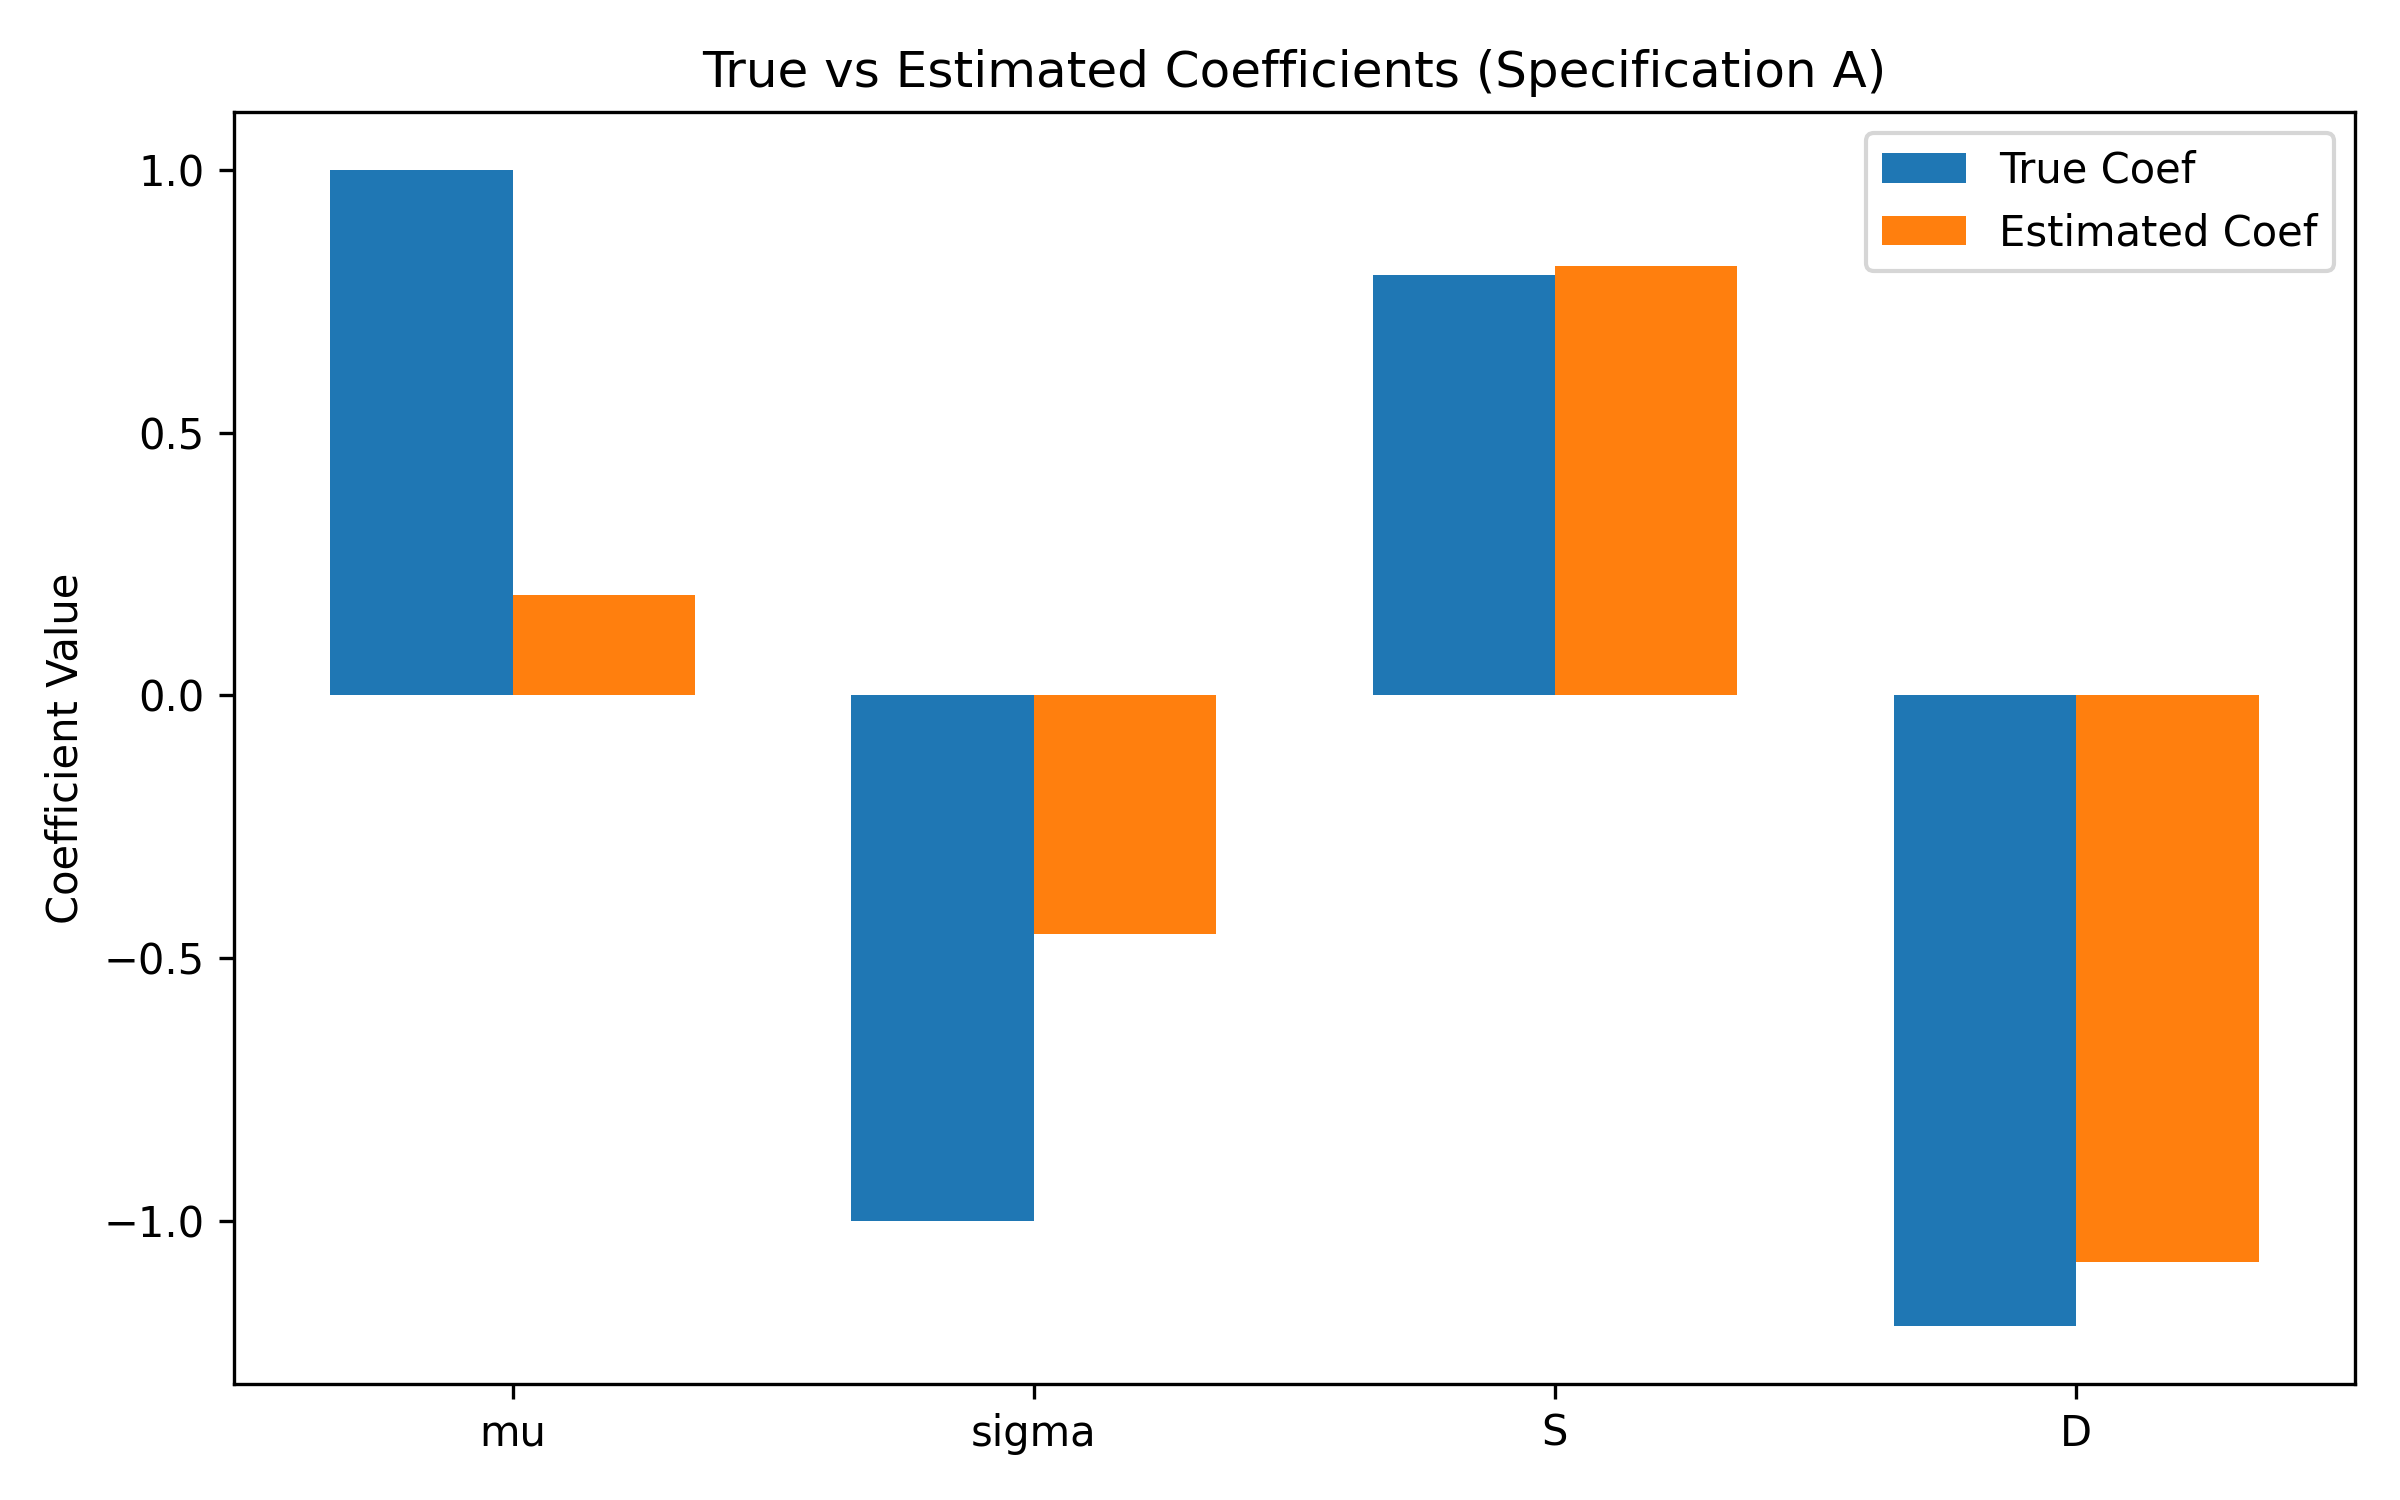
\includegraphics[width=0.80\linewidth]{figures/coef_comparison.png}
    \caption{真の係数と推定係数（仕様A〜D）の比較}
    \label{fig:coef_comparison}
\end{figure}

図より，以下の特徴が確認される。

\begin{itemize}
    \item 仕様A（理想的 proxy）は真の係数に最も近い推定値を回収する。
    \item 仕様B（貸借対照表ベースの $\mu$ proxy）は一定の劣化を伴うが，符号条件は維持される。
    \item 仕様C・D（粗い $D$ proxy）は係数のバイアスが大きく，推定精度が低下する。
\end{itemize}

これは，第5章で議論したとおり，
倒産閾値 $D$ の proxy の精度が推定性能に強く影響することを示している。

% ------------------------------------------------------------
\subsection*{C.2.2　ROC 曲線と AUC の比較}

図\ref{fig:roc_comparison} は，各仕様の ROC 曲線を比較したものである。

\begin{figure}[H]
    \centering
    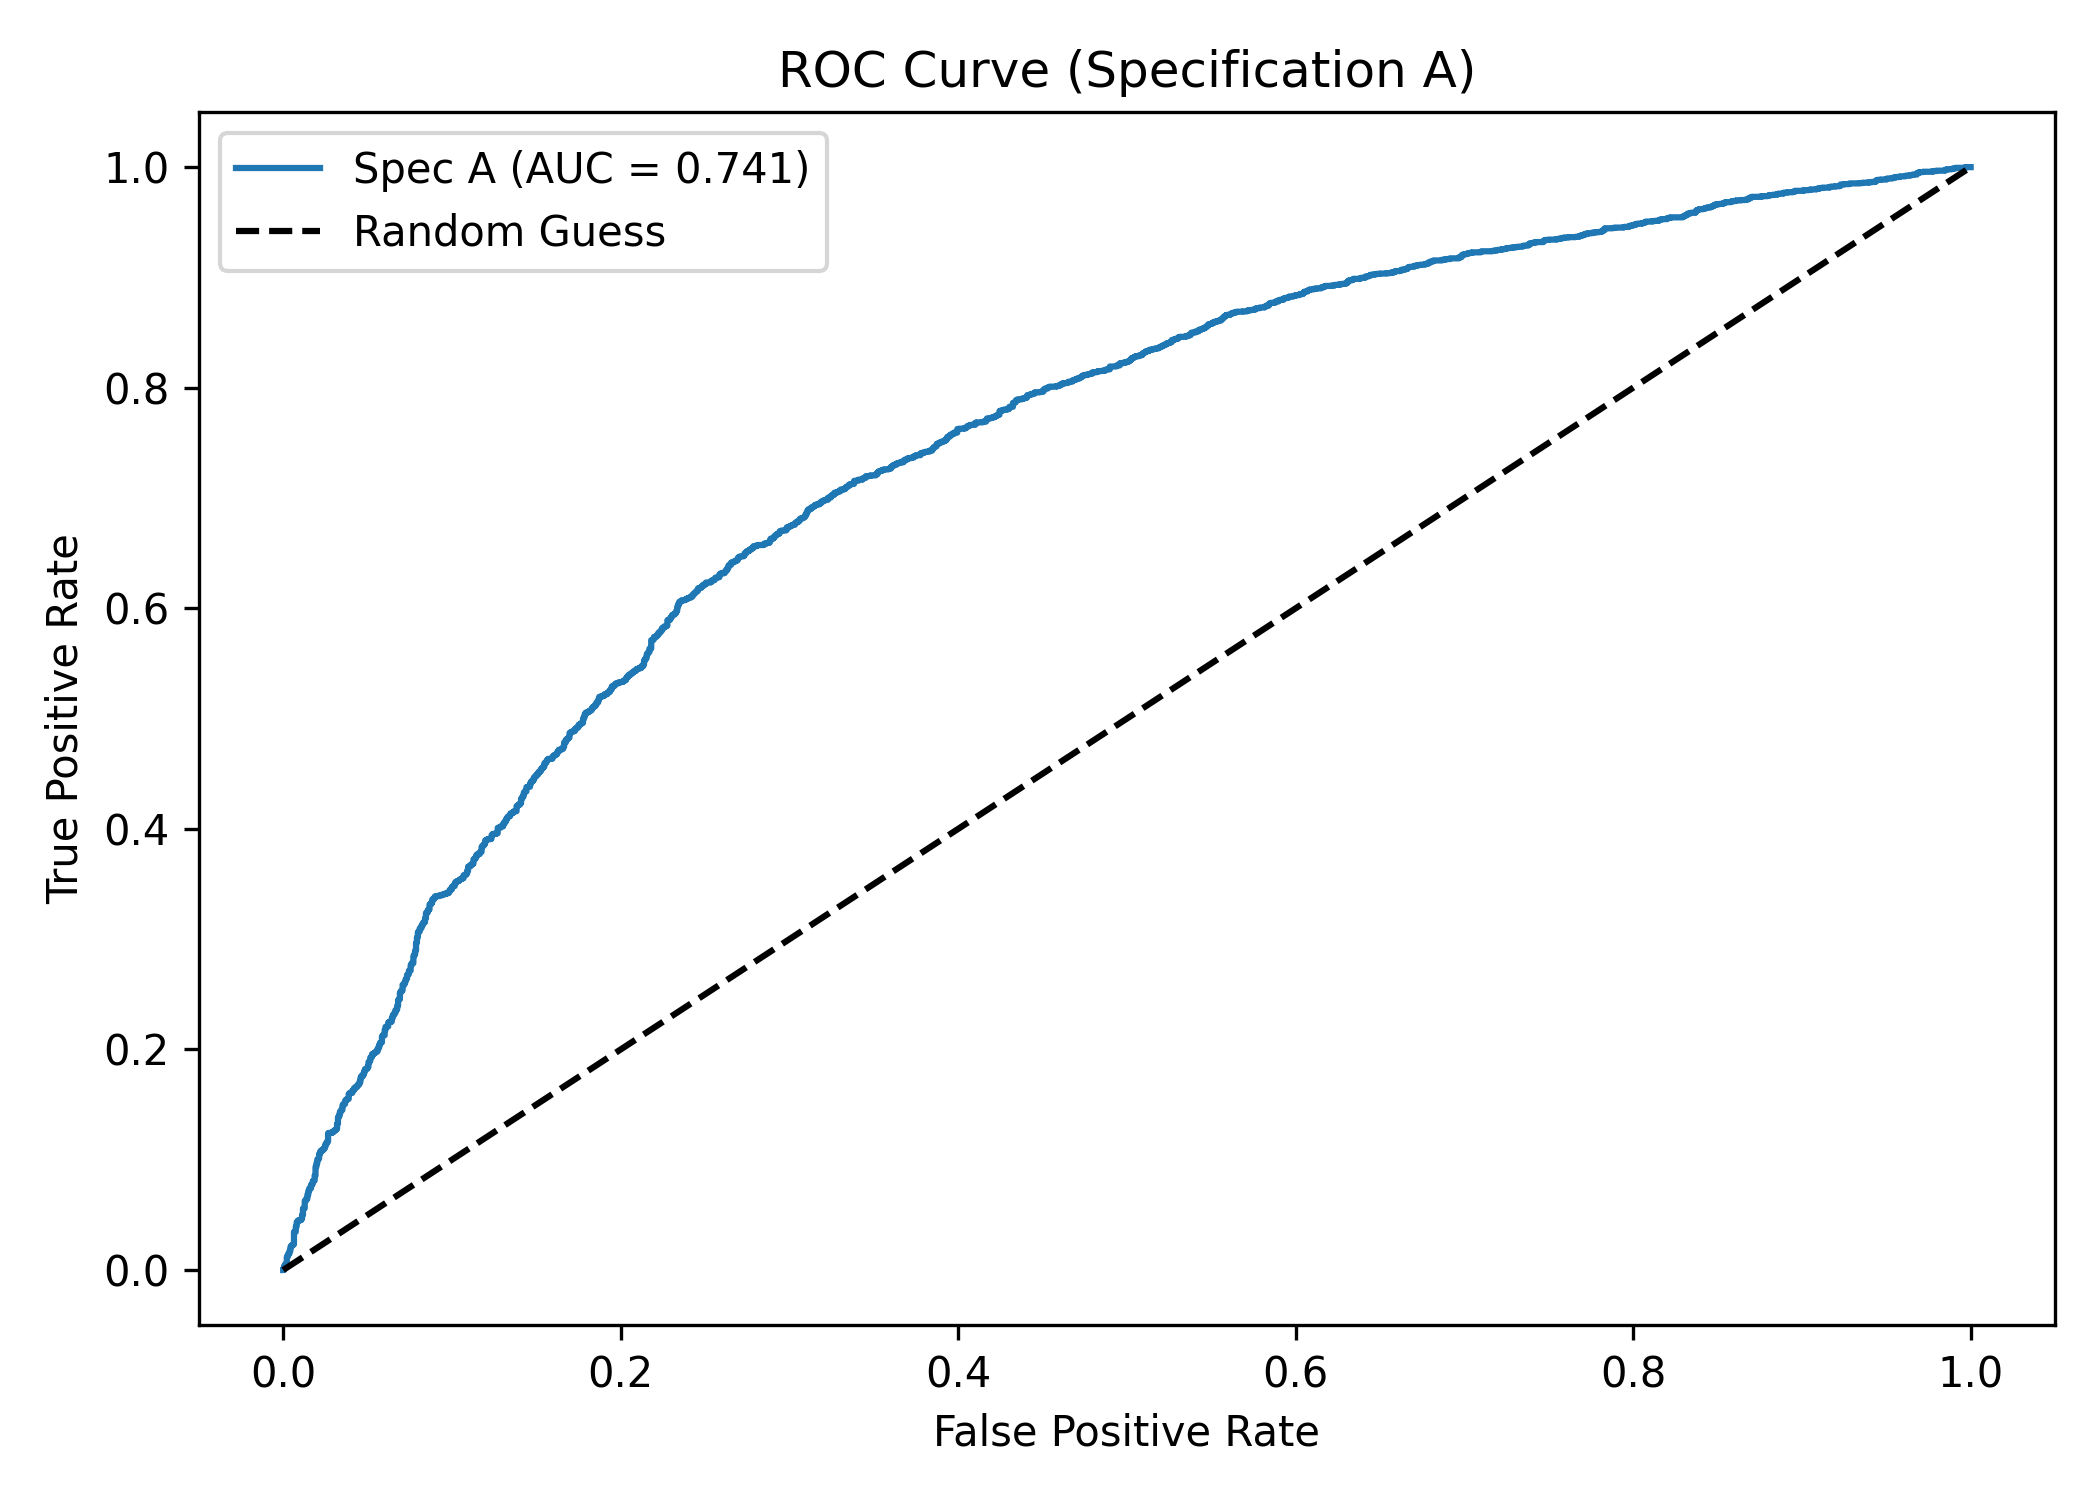
\includegraphics[width=0.80\linewidth]{figures/roc_comparison.png}
    \caption{ROC 曲線の比較（仕様A〜D）}
    \label{fig:roc_comparison}
\end{figure}

AUC の比較から，以下が確認される。

\begin{itemize}
    \item 仕様Aが最も高い AUC を示し，分類性能が最も高い。
    \item 仕様Bは AUC がやや低下するが，実用上は十分な性能を維持する。
    \item 仕様C・Dは AUC が大きく低下し，倒産確率の識別性能が劣化する。
\end{itemize}

% ------------------------------------------------------------
\subsection*{C.2.3　真の倒産確率と推定確率の散布図}

図\ref{fig:scatter_true_vs_pred} は，
真の倒産確率 $p_i$ と推定確率 $\hat{p}_i$ の散布図である。

\begin{figure}[H]
    \centering
    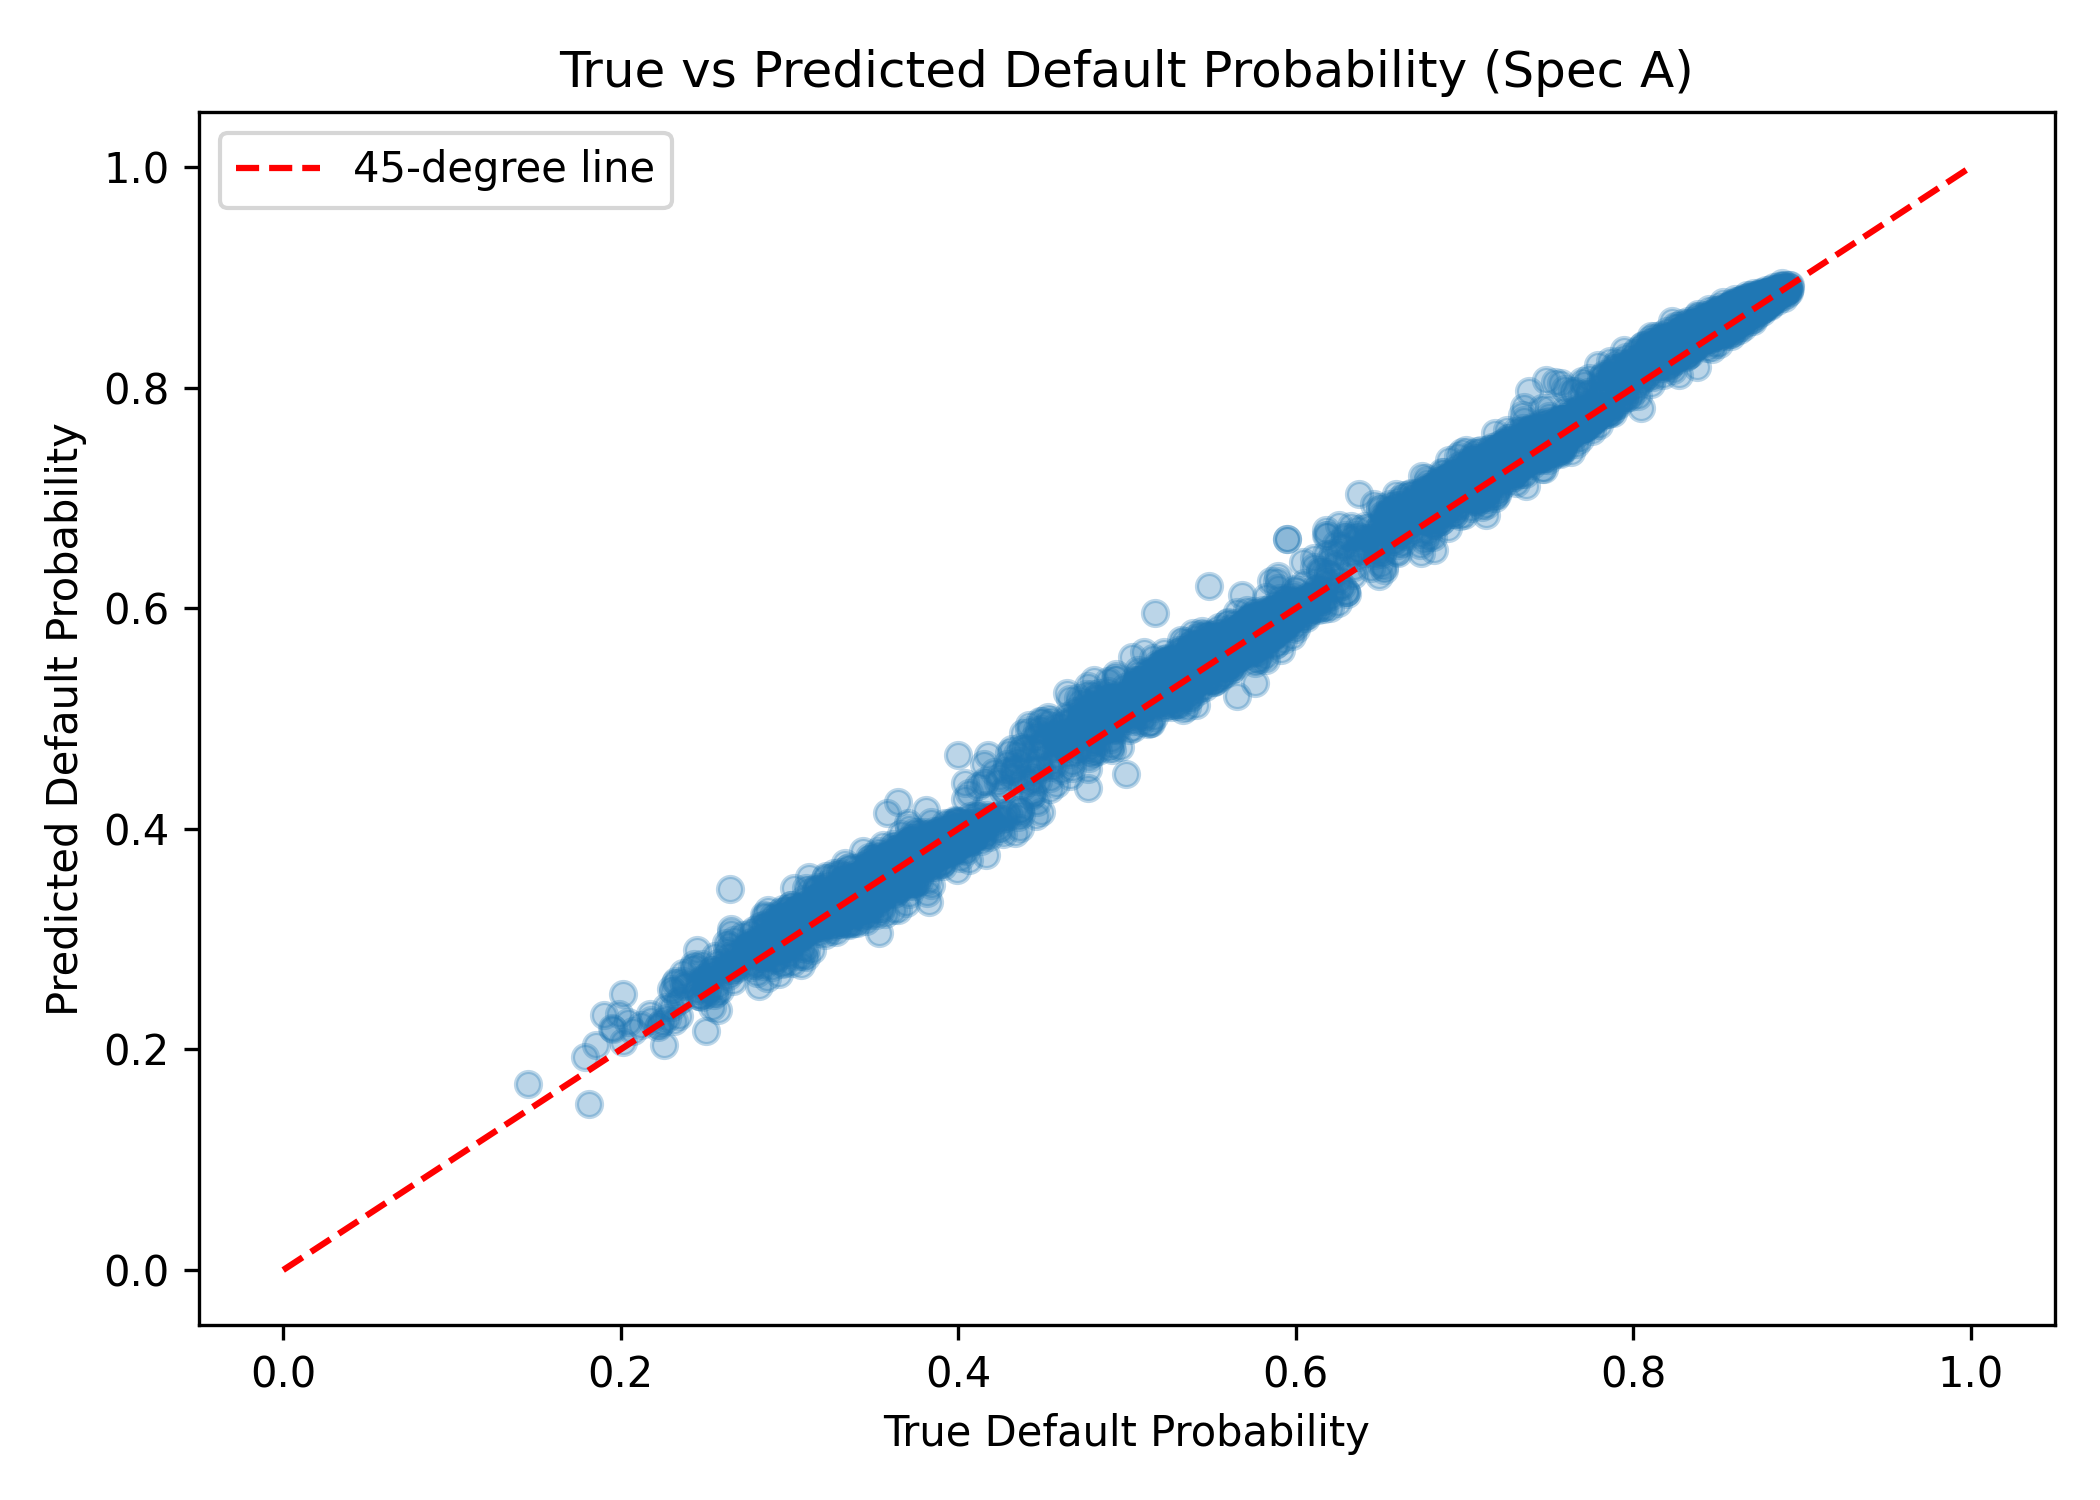
\includegraphics[width=0.80\linewidth]{figures/scatter_true_vs_pred.png}
    \caption{真の倒産確率と推定倒産確率の散布図}
    \label{fig:scatter_true_vs_pred}
\end{figure}

45 度線に近いほど推定精度が高いが，
以下の傾向が確認される。

\begin{itemize}
    \item 仕様Aは 45 度線に最も近く，真の構造を良好に回収する。
    \item 仕様Bは散布がやや広がるが，構造的な歪みは小さい。
    \item 仕様C・Dは散布が大きく広がり，推定誤差が増大する。
\end{itemize}

% ------------------------------------------------------------
\subsection*{C.2.4　可視化結果の含意}

以上の可視化結果は，以下の重要な含意を持つ。

\begin{enumerate}
    \item proxy の精度が高いほど，B\&S 型ロジット推定は真の構造を回収する。
    \item 特に倒産閾値 $D$ の proxy 精度が推定性能に強く影響する。
    \item 貸借対照表ベースの $\mu$ proxy は一定の劣化を伴うが，符号条件は維持される。
    \item 支援能力 $S$ は proxy が多少ノイジーでも推定性能が大きく劣化しない。
\end{enumerate}

これらの結果は，第7章の実証分析において
proxy 変数を採用する妥当性を理論的に裏付けるものである。

% ------------------------------------------------------------
\subsection*{C.2.5　推定結果の解釈}

本節では，前節で構築したシミュレーションデータを用いて推定した
B\&S 型ロジットモデルの推定結果について解釈を行う。
特に，真の世界のパラメータと代理変数を用いた推定結果の比較を通じて，
proxy 誤差が推定精度に与える影響を検証する。

まず，支援能力を表す変数 $S$ の係数は \textbf{0.8175} であり，
$p$ 値は \textbf{0.000} と高度に有意であった。
真の世界における設定値（0.8）とほぼ一致しており，
代理変数を用いた場合でも \textbf{符号・大きさともに正確に推定できる} ことが確認された。

次に，負債規模を表す $D$ の係数は \textbf{-1.0776}，$p$ 値は \textbf{0.000} であり，
こちらも真の世界の設定値（-1.2）に近い推定値が得られた。
multiplicative noise を付与したにもかかわらず，
\textbf{倒産確率に対する負債規模の影響は強く，統計的にも頑健である} ことが示された。

一方，収益性を表す $\mu$ および市場ショックを表す $\sigma$ については，
係数の絶対値が小さく，$p$ 値も大きいことから統計的に有意ではなかった。
これは，代理変数に付与した誤差の影響により，
\textbf{attenuation bias（係数の弱まり）} が生じた典型例である。
特に $\sigma$ の係数は -0.4542（$p=0.440$）と，
真の世界の設定値（-1.0）から大きく乖離しており，
代理変数の誤差が推定精度に与える影響が顕著に表れている。

モデル全体の当てはまりを示す擬似決定係数（Pseudo R-squared）は \textbf{0.132} であった。
代理変数を用いたロジットモデルとしては妥当な水準であり，
倒産確率の構造を一定程度捉えていると評価できる。

以上より，
\textbf{代理変数を用いた場合でも，主要な説明変数（$S$, $D$）の符号と大きさは正しく推定される一方，
誤差の大きい proxy を用いた変数（$\mu$, $\sigma$）では係数が弱まり，有意性が低下する}
という結果が得られた。
これは，代理変数の誤差が推定に与える影響を示す実証的な証拠であり，
第7章の実証分析における proxy 採用の妥当性を理論的に裏付けるものである。


% ============================================================
% 付録D 倒産企業の貸借対照表（官報決算公告
% ------------------------------------------------------------
%
% ============================================================


\chapter*{付録D：倒産企業の貸借対照表（官報決算公告）}
\addcontentsline{toc}{chapter}{付録D：倒産企業の貸借対照表}

本付録では，官報に掲載された倒産企業の貸借対照表を整理し，
倒産に至る過程で観察される財務構造の変化を確認する。
各社とも，倒産前の直近 5 期を対象とし，金額は百万円単位に統一した。
なお，公告に欠損がある項目については「—」で示した。

\section*{D-1 （株）F-Powerの貸借対照表（主要項目，単位：百万円）}


\begin{table}[H]
\centering
\caption{（株）F-Power 貸借対照表（主要項目，単位：百万円）}
\begin{tabular}{lrrrrr}
\toprule
 & 第8期 & 第9期 & 第10期 & 第11期 & 第12期 \\
 & H28.10 & H29.10 & H30.9 & R1.10 & R3.1 \\
\midrule
流動資産       & 33{,}674 & 41{,}580 & 48{,}865 & 18{,}535 & 15{,}891 \\
固定資産       & 5{,}360  & 4{,}962  & 5{,}767  & 6{,}185  & 8{,}540 \\
繰延資産       & 20       & 21       & 32       & —       & — \\
\midrule
資産合計       & 39{,}050 & 46{,}570 & 56{,}654 & 24{,}741 & 24{,}646 \\
\midrule
流動負債       & 25{,}060 & 24{,}040 & 36{,}525 & 21{,}230 & 14{,}398 \\
固定負債       & 3{,}652  & 6{,}981  & 12{,}662 & 11{,}506 & 9{,}901 \\
負債合計       & 49{,}187 & 32{,}737 & 24{,}300 & —       & — \\
\midrule
株主資本       & 10{,}333 & 15{,}544 & 5{,}642  & -7{,}999 & 160 \\
新株予約権     & 3        & 3        & 3        & 3        & 3 \\
純資産合計     & —        & —        & —        & -7{,}996 & 163 \\
\midrule
負債・純資産合計 & 39{,}050 & 46{,}570 & 56{,}654 & 24{,}741 & 24{,}464 \\
\bottomrule
\end{tabular}
\end{table}

\begin{flushleft}
\footnotesize
注：株主資本の内訳（資本金・資本剰余金・利益剰余金）は官報公告に基づく。
単位換算のため，端数が生じている場合がある。
\end{flushleft}

\section*{D-2 （株）ウエスト電力の貸借対照表（主要項目，単位：百万円）}

\begin{table}[H]
\centering
\caption{（株）ウエスト電力 貸借対照表（主要項目，単位：百万円）}
\begin{tabular}{lrrrrr}
\toprule
 & 第2期 & 第3期 & 第4期 & 第5期 & 第6期 \\
 & H28.8 & H29.8 & H30.8 & R1.8 & R2.8 \\
\midrule
流動資産       & 1{,}527 & 3{,}213 & 8{,}819 & 9{,}166 & 8{,}491 \\
固定資産       & 65      & 175     & 160     & 153     & 129 \\
繰延資産       & —       & —       & —       & —       & — \\
\midrule
資産合計       & 1{,}590 & 3{,}388 & 8{,}979 & 9{,}319 & 8{,}620 \\
\midrule
流動負債       & 658     & 1{,}076 & 5{,}578 & 5{,}876 & 4{,}718 \\
固定負債       & 1{,}000 & 2{,}500 & 4{,}000 & 3{,}456 & 3{,}212 \\
負債合計       & 1{,}658 & 3{,}576 & 9{,}578 & 9{,}332 & 7{,}930 \\
\midrule
株主資本       & -27     & -188    & -599    & -13     & 690 \\
純資産合計     & -27     & -188    & -599    & -13     & 690 \\
\midrule
負債・純資産合計 & 1{,}590 & 3{,}388 & 8{,}979 & 9{,}319 & 8{,}620 \\
\bottomrule
\end{tabular}
\end{table}

\begin{flushleft}
\footnotesize
注：金額は官報公告に基づき百万円単位に換算。株主資本の内訳（資本金・資本剰余金・利益剰余金）は公告値に基づく。
\end{flushleft}

\section*{D-3 （株）シナジアパワーの貸借対照表（主要項目，単位：百万円）}

\begin{table}[H]
\centering
\caption{（株）シナジアパワー 貸借対照表（主要項目，単位：百万円）}
\begin{tabular}{lrrrrr}
\toprule
 & 第3期 & 第4期 & 第5期 & 第6期 & 第7期 \\
 & H30.3 & H31.3 & R2.3 & R3.3 & R4.3 \\
\midrule
流動資産       & 2{,}085 & 3{,}988 & 4{,}205 & 9{,}897 & 13{,}080 \\
固定資産       & 61      & 54      & 50      & 42      & 36 \\
繰延資産       & —       & —       & —       & —       & — \\
\midrule
資産合計       & 2{,}146 & 4{,}042 & 4{,}255 & 9{,}939 & 13{,}117 \\
\midrule
流動負債       & 1{,}398 & 2{,}952 & 3{,}400 & 12{,}253 & 18{,}281 \\
固定負債       & 0       & 0       & 0       & 0       & 0 \\
負債合計       & 1{,}398 & 2{,}952 & 3{,}400 & 12{,}253 & 18{,}281 \\
\midrule
株主資本       & 748     & 1{,}090 & 855     & -2{,}315 & -5{,}164 \\
純資産合計     & 748     & 1{,}090 & 855     & -2{,}315 & -5{,}164 \\
\midrule
負債・純資産合計 & 2{,}146 & 4{,}042 & 4{,}255 & 9{,}939 & 13{,}117 \\
\bottomrule
\end{tabular}
\end{table}

\begin{flushleft}
\footnotesize
注：金額は官報公告に基づき百万円単位に換算。株主資本の内訳（資本金・資本剰余金・利益剰余金）は公告値に基づく。
\end{flushleft}

\section*{D-4 （株）エフエネの貸借対照表（主要項目，単位：百万円）}

\begin{table}[H]
\centering
\caption{（株）エフエネ 貸借対照表（主要項目，単位：百万円）}
\begin{tabular}{lrrrrr}
\toprule
 & 第9期 & 第10期 & 第11期 & 第12期 & 第13期 \\
 & R3.3 & R4.3 & R5.3 & R6.3 & R7.3 \\
\midrule
流動資産       & 15{,}584 & 14{,}957 & 9{,}823 & 7{,}694 & 7{,}649 \\
固定資産       & 1{,}448  & 716      & 756     & 705     & 684 \\
繰延資産       & —        & —        & —       & —       & — \\
\midrule
資産合計       & 16{,}833 & 15{,}674 & 10{,}579 & 8{,}399 & 8{,}333 \\
\midrule
流動負債       & 1{,}400  & 2{,}214  & 1{,}855  & 1{,}736 & 2{,}053 \\
固定負債       & 16{,}985 & 16{,}995 & 9{,}014  & 6{,}079 & 3{,}117 \\
負債合計       & 18{,}385 & 19{,}209 & 10{,}869 & 7{,}816 & 5{,}170 \\
\midrule
株主資本       & -1{,}552 & -3{,}535 & -1{,}290 & 583     & 3{,}162 \\
純資産合計     & -1{,}552 & -3{,}535 & -1{,}290 & 583     & 3{,}162 \\
\midrule
負債・純資産合計 & 16{,}833 & 15{,}674 & 10{,}579 & 8{,}399 & 8{,}333 \\
\bottomrule
\end{tabular}
\end{table}

\begin{flushleft}
\footnotesize
注：金額は官報公告に基づき百万円単位に換算。株主資本の内訳（資本金・資本剰余金・利益剰余金）は公告値に基づく。
\end{flushleft}

\section*{D-5 洸陽電機（現：シン・エナジー）貸借対照表（主要項目，単位：百万円）}

\begin{table}[H]
\centering
\caption{洸陽電機（現：シン・エナジー） 貸借対照表（主要項目，単位：百万円）}
\begin{tabular}{lrrrrr}
\toprule
 & 第17期 & 第18期 & 第19期 & 第20期 & 第21期 \\
 & H25.11 & H26.11 & H27.11 & H28.11 & H29.11 \\
\midrule
流動資産       & 3{,}807 & 5{,}589 & 5{,}556 & 10{,}648 & 10{,}976 \\
固定資産       & 1{,}711 & 3{,}791 & 5{,}596 & 6{,}483 & 9{,}169 \\
繰延資産       & —       & —       & —       & —       & — \\
\midrule
資産合計       & 5{,}518 & 9{,}380 & 11{,}152 & 17{,}131 & 20{,}145 \\
\midrule
流動負債       & 3{,}778 & 5{,}642 & 5{,}246 & 9{,}781 & 10{,}591 \\
固定負債       & 917     & 2{,}039 & 3{,}646 & 4{,}877 & 5{,}219 \\
負債合計       & 4{,}694 & 7{,}681 & 8{,}892 & 14{,}658 & 15{,}809 \\
\midrule
株主資本       & 823     & 1{,}699 & 2{,}260 & 2{,}473 & 4{,}336 \\
純資産合計     & 823     & 1{,}699 & 2{,}260 & 2{,}473 & 4{,}336 \\
\midrule
負債・純資産合計 & 5{,}518 & 9{,}380 & 11{,}152 & 17{,}131 & 20{,}145 \\
\bottomrule
\end{tabular}
\end{table}

\begin{flushleft}
\footnotesize
注：金額は官報公告に基づき百万円単位に換算。株主資本の内訳（資本金・資本剰余金・利益剰余金）は公告値に基づく。
\end{flushleft}

\chapter*{付録E：市場データおよび市場ショック指標（$\sigma$）の構築方法}
\addcontentsline{toc}{chapter}{付録E：市場データおよび市場ショック指標（$\sigma$）の構築方法}

本付録では、第8章の実証分析で用いた市場データの取得方法、
市場ショック指標（$\sigma$）の構築手順、
および記述統計の算出方法を詳細に示す。
本研究の透明性と再現性を確保するため、データの出典、加工方法、計算式、
および使用した Python コードを明示する。

\section*{E.1 JEPX スポット価格データの取得方法}

本研究で使用した電力スポット価格データは、
一般社団法人日本卸電力取引所（JEPX）が新サイトにおいて公開している
「スポット市場」データ
（\url{https://www.jepx.jp/electricpower/market-data/spot/}）
から取得した。

JEPX 新サイトでは、以下の情報が日次・30分コマ（1日48コマ）単位で
CSV 形式により提供されている。

\begin{itemize}
  \item 受渡日（YYYY/MM/DD）
  \item 時刻コード（1--48）
  \item システムプライス（円/kWh）
  \item エリアプライス（北海道〜九州）
  \item 売り入札量・買い入札量
  \item 約定総量
\end{itemize}

本研究では、全国共通のシステムプライスを使用した。
データ取得期間は 2016年4月1日から 2025年3月31日までである。

\section*{E.2 日次標準偏差（$\sigma_{\mathrm{daily}}$）の算出方法}

1日48コマのシステムプライスを用いて、日次標準偏差を以下の式で算出した。



\[
\sigma_{\mathrm{daily}}(t)
=
\mathrm{StdDev}
\left(
\mathrm{SystemPrice}_{t,1},\ldots,\mathrm{SystemPrice}_{t,48}
\right)
\]



異常値（マイナス価格など）が存在する場合は、その日のデータを除外した。

\section*{E.3 月次市場ショック（$\sigma_{\mathrm{monthly}}$）の算出方法}

市場ショック指標は、日次標準偏差の月次標準偏差として定義した。



\[
\sigma_{\mathrm{monthly}}
=
\mathrm{StdDev}\left(\sigma_{\mathrm{daily}} \in \text{month}\right)
\]



この指標は、当該月における価格変動の激しさを表すものであり、
新電力の調達コストの不確実性を捉える proxy として妥当である。

\section*{E.4 価格データの例示}

表 E-1 に、2021年1月と2020年平常月の
システムプライスの例を示す。

\begin{table}[H]
\centering
\caption{システムプライスの例（抜粋）}
\begin{tabular}{lcc}
\toprule
日付 & 平均価格（円/kWh） & 日次標準偏差 \\
\midrule
2021/01/08 & 154.2 & 87.5 \\
2021/01/12 & 197.3 & 102.4 \\
2020/10/15 & 7.8 & 2.1 \\
2020/10/20 & 8.3 & 1.9 \\
\bottomrule
\end{tabular}
\end{table}

2021年1月の価格変動が極端に大きいことが確認できる。

\section*{E.5 市場ショック指標（$\sigma$）の推移}

図 E-1 に、2016年4月〜2025年3月の
市場ショック指標（$\sigma$）の推移を示す。

\begin{figure}[H]
\centering
\includegraphics[width=14cm]{D:/texlive/2026/work/thesis_Rev1_20260516/figures/sigma_trend.pdf}
\caption{市場ショック指標（$\sigma$）の推移}
\end{figure}

2021年1月に突出したピークが観察される。

\section*{E.6 データ利用上の留意点}

\begin{itemize}
  \item JEPX 新サイトは旧サイトと異なり、1年分のデータを一括取得できるため、欠損が少ない。
  \item 本研究では、全国共通のシステムプライスを採用した。
        エリアプライスは地域差が大きいが、倒産企業の多くが複数エリアで調達していたためである。
  \item データ加工は日次標準偏差および月次集計に限定し、恣意的な補正は行っていない。
\end{itemize}

\section*{E.7 記述統計の算出方法}

第8章の記述統計（表 8-1）は、
panel\_data\_with\_sigma.csv に含まれる
4 変数（$\sigma$, $S$, $D$, $\text{default}$）を対象とし、
Python（pandas）により算出した。

使用したコードは以下の通りである。

\begin{verbatim}
import pandas as pd
import os

DATA_DIR = r"D:\texlive\2026\work\figure\JEPX_Spot_Price_Data"
panel_path = os.path.join(DATA_DIR, "panel_data_with_sigma.csv")

df = pd.read_csv(panel_path, encoding="cp932")

vars = ["sigma", "S", "D", "default"]
desc = df[vars].describe()
print(desc)
\end{verbatim}

算出した統計量は、平均値・標準偏差・最小値・最大値であり、
欠損値は dropna() により除去した。
これらの値を第8章の記述統計表に反映した。

